\documentclass[a4paper,12pt,oneside]{report}
\usepackage{OvidiusFMI}
\usepackage{times}
\usepackage{graphicx}
\usepackage{hyperref}
\usepackage{color,xcolor}
\usepackage{amsmath}
\usepackage{framed}
\usepackage{indentfirst}
\usepackage{enumerate}
\usepackage[shortlabels]{enumitem}
\usepackage{listings}
\usepackage{amsmath,amsfonts,amssymb,amsthm,epsfig,epstopdf,url,array}
\usepackage{multicol,multirow}
\definecolor{code}{rgb}{0.97,0.97,0.97}
\lstdefinestyle{customc}{
  belowcaptionskip=1\baselineskip,
  backgroundcolor=\color{code},
  breaklines=true,
%  frame=L,
%  xleftmargin=\parindent,
  language=C,
  showstringspaces=false,
  morekeywords={bool,
  				 glutMainLoop, glutIdleFunc, glMatrixMode, glLoadIdentity, glPushMatrix, glPopMatrix, 
  				 glBegin, glEnd, glTranslatef, glRotatef, glScalef, glColor3f, glColor4f, glutSolidCube, glutWireCube, glutSolidSphere,
  				 glutWireSphere, glutSolidCone,glutSetWindowTitle,glutGet,glClear,glutSwapBuffers,glDepthFunc,
  				 glutWireCone, glutSolidTorus, glutWireTorus, glutSolidDodecahedron, glutWireDodecahedron,
  				 glutSolidOctahedron, glutWireOctahedron, glutSolidTetrahedron, glutWireTetrahedron, 
  				 glVertex3f,glVertex2f,glPointSize,
  				 glutSolidIcosahedron, glutWireIcosahedron, glutSolidTeapot, glutWireTeapot,glutReshapeFunc,
  				 glFlush, gluPerspective, glutPostRedisplay, glutInit, glutKeyboardFunc,glutKeyboardUpFunc,
  				 glutInitWindowSize, glutInitWindowPosition, glutInitDisplayMode, glutCreateWindow, glutDisplayFunc,glutPassiveMotionFunc,
  				 glClear,glTexCoord2f,
  				 glEnable, glDisable, glLightfv, glMaterialfv, glCullFace,glViewport,
  				 glFrontFace,glColor3ub, glShadeModel,
  				 glGenLists, glGetFloatv,glGentextures,glTexImage2D,glTexParameteri, free, glDeleteTextures,
  				 glLineStipple, glLineWidth, glBindTexture,glGenTextures,
  				 glNewList, glEndList, glCallList,
  				 glMap1f,glEvalCoord1f,glMapGrid1d,glEvalMesh1,glMap2f,glEvalCoord2f,glMapGrid2f,glEvalMesh2,
  				 gluBeginTrim, gluEndTrim, gluPwlCurve,glHint,
  				 GLUnurbsObj, gluBeginSurface, gluNurbsSurface, gluEndSurface, gluNewNurbsRenderer, 									gluNurbsProperty,gluQuadricNormals,
  				 glNormal3f,
  				 gluQuadricTexture,GLUquadricObj,gluSphere,
  				 glPolygonMode, glBlendFunc,glFogi,glFogiv,glFogfv,
  				 GLfloat, GLdouble, GLint,GLuint, GLushort,GLubyte, glRasterPos2f,
  				 gluBeginCurve, gluNurbsCurve, gluEndCurve,
  				 glOrtho, gluLookAt, glutBitmapCharacter, 
  				 glInitNames, glPushName, glLoadName, glSelectBuffer, glRenderMode,gluPickMatrix, glGetIntegerv, glutMouseFunc,glutMotionFunc,system,
  				 glPushAttrib, glPopAttrib, glMultMatrixf, sprintf, glClearStencil, glStencilFunc,glStencilOp,glStencilMask,glColorMask,glActiveStencilFaceEXT,fprintf},  
%   numbers=left,                    % where to put the line-numbers; possible values are (none, left, right)
  %numbersep=5pt,                   % how far the line-numbers are from the code
  %numberstyle=\tiny\color{code}, % the style that is used for the line-numbers
  basicstyle=\footnotesize\ttfamily,
  keywordstyle=\bfseries\color{green!40!black},
  commentstyle=\itshape\color{purple!40!black},
  identifierstyle=\color{blue},
  stringstyle=\color{orange},
}

\lstset{escapechar=@,style=customc}


\newtheorem{definition}{Defini\c tie}
\newtheorem{problem}{Problema}
\newtheorem{proposition}{Propozi\c tie}
\newtheorem{demonstration}{Demonstra\c tie}
\newtheorem{example}{Exemplu}
\newtheorem{theorem}{Teorem\u a}
\newtheorem{remark}{Observa\c{t}ie}
\newtheorem{lemma}{Lem\u{a}}
\newtheorem{solve}{Rezolvare}
\newtheorem{corollary}{Corolar}
\renewcommand*{\proofname}{\rm\bf{Demonstra\c{t}ie}:}

\facultatea{Matematic\u a \c si Informatic\u a}
\specializarea{Informatic\u a}
\teza{Diserta\c{t}ie}
\titlu{Func\c{t}ii convexe. Aplica\c{t}ii  }
\coordonatorPrincipal{Prof. univ. Cosma Lumini\c ta}
\autor{T\u anase Ramona Elena}
\data{2022}

\begin{document}
\maketitle

\pagenumbering{roman}
\tableofcontents
\listoffigures

\newpage
\pagenumbering{arabic}


\chapter*{Abstract}

Convexitatea este o no\c{t}iune simpl\u{a} \c{s}i natural\u{a} care dateaz\u{a} \^{i}nc\u{a} de la Arhimede (circa 250 \^{i}.e.n.), \c{s}i are leg\u{a}tur\u{a} cu celebra sa estimare a valorii lui \(\pi\) (prin folosirea poligoanelor regulate \^{i}nscrise \c{s}i circumscrise).

Recunoa\c{s}terea subiectului func\c{t}iilor convexe este \^{i}n general atribuit\u{a} lui J. L. W. V. Jensen. Cu toate acestea, nu a fost primul care s-a ocupat de astfel de func\c{t}ii. Printre predecesorii s\u{a}i \^{i}i putem aminti pe Ch. Hermite, O. Hölder \c{s}i O. Stolz.

Din ce \^{i}n ce mai mul\c{t}i matematicieni folosesc convexitatea ca pe o modalitate de a dezv\u{a}lui adev\u{a}rata natur\u{a} a anumitor probleme complicate. Exist\u{a} dou\u{a} propriet\u{a}\c{t}i de baz\u{a} ale func\c{t}iilor convexe care le fac at\^{a}t de utilizate pe scar\u{a} larg\u{a} \^{i}n matematica teoretic\u{a} \c{s}i aplicat\u{a}. Pe de o parte una dintre propriet\u{a}\c{t}i arat\u{a} faptul c\u{a} maximul este atins \^{i}ntr-un punct de limit\u{a}. Pe de alt\u{a} parte, orice minim local este unul global. Mai mult, o func\c{t}ie strict convex\u{a} admite cel mult un minim.

Convexity is a simple and  natural notion that dates back to Archimedes (about
250 BC), and is related to his famous estimate of the value of \(\pi\)  (by using polygons
regular and circumscribed).

Recognition of the subject of convex functions is generally attributed to J. L. W. V.
Jensen. However, he was not the first to hold such positions. Among the prey we can remember Ch. Hermite, O. Hölder and O. Stolz.

More and more mathematicians are using convexity as a way to
reveal the true nature of certain complicated problems. There are two basic properties
of the convex functions that make them so widely used in theoretical and applied mathematics. On the one hand, one of the properties shows that the maximum is reached at a point
of limit. On the other hand, any local minimum is a global one. Moreover, a strict function
convex admits at least a minimum.

\chapter*{Introducere}


Convexitatea este un subiect  vechi \^{i}n matematic\u{a}. Prima defini\c{t}ie specific\u{a} a convexit\u{a}\c{t}ii
a fost dat de Herman Minkowski \^{i}n 1896. Func\c{t}iile convexe au fost introduse de Jensen
\^{i}n 1905. Conceptul a ap\u{a}rut intermitent de-a lungul secolelor, dar subiectul
nu a fost \^{i}ntr-adev\u{a}r oficializat p\^{a}n\u{a} \^{i}n 1934.

De fapt, experiment\u{a}m convexitatea tot timpul \c{s}i \^{i}n multe feluri. Cel mai prozaic exemplu este pozi\c{t}ia noastr\u{a} vertical\u{a}, care este asigurat\u{a} at\^{a}ta timp c\^{a}t proiec\c{t}ia vertical\u{a} a centrului nostru de greutate se afl\u{a} \^{i}n interiorul \^{i}nveli\c{s}ului convex al picioarelor noastre.De asemenea, convexitatea are un impact mare asupra vie\c{t}ii noastre de zi cu zi prin numeroase aplica\c{t}ii \^{i}n industrie, afaceri, medicin\u{a} \c{s}i art\u{a}.

\^{I}mi propun ca , prezenta lucrare, s\u{a} fie o introducere \^{i}n convexitatea func\c{t}iilor, pornind de la defini\c{t}ia unei func\c{t}ii covexe \c{s}i propriet\u{a}\c{t}ile sale,  Inegalitatea lui Jenssen \c{s}i Inegalitatea ui Young\c{s}i nu \^{i}n ultimul r\^{a}nd Inegalitatea Cauchy-Bunyakovsky-Schwars.

\^{I}n primul capitol vom discuta despre convexitatea func\c{t}iilor, opera\c{t}ii cu func\c{t}ii ocnvexe dar \c{s}i inegalit\u{a}\c{t}i ale acestora. Vom prezenta inegalitatea lui Jensen, forma ponderata a inegalit\u{a}\c{t}ii mediilor, urmat\u{a} de inegalitatea lui Young \c{s}i consecin\c{t}ele sale: inegalitatea lui Rogers-Holder pentru p \(>\) 1, inegalitatea Cauchy-Bunyakovsky-Schwarz \c{s}i nu \^{i}n ultimul r\^{a}nd inegalitatea Minkowski \c{s}i derivabilitatea func\c{t}iilor convexe.

Cel de al doilea capitol prezint\u{a} aplica\c{t}ii ale func\c{t}iilor convexe. Printre acestea vom reg\u{a}si: Problema asupra produsului maxim a dou\u{a} laturi \^{i}ntr-un triunghi, Formula defectului lui Hölder - acest rezultat provine din faimoasa lucrare a lui Otto Ludwig Hölder \^{i}n care se g\u{a}seşte demonstra\c{t}ia inegalit\u{a}ţii care are a ajuns s\u{a} fie cunoscut\u{a}  ca ”inegalitatea lui Hölder”. Formula defectului 
\begin{displaymath}
      \sum_{k = 1}^{n}p_{k}f\left ( x_{k} \right ) - f\left ( \sum_{k = 1}^{n} p_{k}x_{k}\right ) = \frac{1}{4}\mu \sum_{j = 1}^{n}\sum_{k = 1}^{n}p_{j}p_{k}\left ( x_{j} - x_{k} \right )^{2}.
\end{displaymath}
este mult mai pu\c{t}in cunoscut\u{a}, dar este totu\c{s}i valoroas\u{a}, precum \c{s}i  inegalitatea ariei n-poligonului, supraaditivitatea mediei geometrice dar \c{s}i Criteriul derivatei secunde \c{s}i Teorema lui Rolle.


%
%
%CAPITOLUL 1
%
%
\chapter{No\c{t}iuni teoretice}

\section{Defini\c{t}ii. Propriet\u{a}\c{t}i}

\nocite{niculescu}
\nocite{marasanu}

Studiul func\c{t}iilor convexe de o variabil\u {a} reala\u {a}, ofer\u{a} o imagine excelent\u {a} a frumuse\c {t}ii \c{s}i fascina\c{t}iei matematicii avansate. Vom g\u{a}si aici o mare varietate de rezultate bazate pe argumente simple \c{s}i intuitive care au aplica\c{t}ii remarcabile.

\^{I}n continuare vom nota cu I un interval nedegenerat din \(\mathbb{R}\).

\begin{definition}

O functie \(f: I \rightarrow \mathbb{R}\) se nume\c{s}te convex\u{a} dac\u{a},
\begin{displaymath}
f \left ( \left ( 1 - \lambda  \right )x + \lambda y \right )\leq \left ( 1 - \lambda  \right ) f_{\left ( x \right )} + \lambda f_{\left ( y \right )}   \label{eq:1.1} \tag{1.1}
\end{displaymath}
pentru orice \(x\) \c{s}i \(y\) din \(I\), \c{s}i orice \(\lambda \in \left [ 0,1 \right ]\). Func\c{t}ia \(f\) se nume\c{s}te strict convex\u{a} dac\u{a} inegalitatea \ref{eq:1.1} se pastreaz\u{a}  strict\u{a} pentru orice x \c{s}i y din I, \c{s}i orice  \(\lambda \in \left ( 0,1 \right )\) . Dac\u{a} \(-f\) este convex\u{a} (respectiv stric convex\u{a}), atunci spunem c\u{a} \(f\) este concav\u{a} (respectiv strict concav\u{a}). Dac\u{a} \(f\) este \c{s}i convex\u{a} \c{s}i concav\u{a}, atunci spunem c\u{a} \(f\) este func\c{t}ie afin\u{a}.
\end{definition}

Func\c{t}iile afine sunt tocmai func\c{t}iile de forma \(mx + n\),  \(m\) \c{s}i \(n\) constante reale.
Se poate demonstra u\c{s}or faptul c\u{a} primele trei func\c{t}ii sunt convexe (dar nu sunt strict convexe) iar celelalte dou\u{a} sunt strict convexe, respectiv strict concave:
\begin{enumerate}
  \item partea pozitiv\u{a} \(x^{+} = max \left \{ x,0 \right \}\),
  \item partea negativ\u{a} \(x^{-} = max \left \{ -x,0 \right \}\),
  \item modulul \(\left | x \right | = max \left \{ -x,x \right \}\),
  \item func\c{t}ia p\u{a}tratic\u{a} \(x^{2}\)  este strict convex\u{a} pe \(\mathbb{R}\),
  \item func\c{t}ia r\u{a}d\u{a}cin\u{a} p\u{a}trat\u{a} \(\sqrt{x}\) este strict concav\u{a} pe \(\mathbb{R}_{+}\).
\end{enumerate}

Alte criterii de convexitate legate de teoria de baz\u{a} a func{t}iilor convexe vor fi prezentate \^{i}n cele ce urmeaz\u{a}.\\

Convexitatea unei func\c{t}ii \(f : I\rightarrow \mathbb{R}\), \^{i}nseamn\u{a} geometric faptul c\u{a}, punctele de pe graficului lui  \(f|_{\left [ u,v \right ]}\) sunt sub (sau pe) coarda care une\c{s}te capetele \(\left ( u , f {\left ( u \right )} \right )\)  \c{s}i \(\left ( v , f {\left ( v \right )} \right )\) pentru orice \(u, v \in I, u < v\);
(vezi Fig 1.1).

Astfel inegalitatea \ref{eq:1.1} este echivalent\u{a} cu:
\begin{displaymath}
  f\left ( x \right )\leq f\left ( u \right ) +\frac{f\left ( v \right )- f\left ( u \right )}{v - u}\left ( x - u \right ) \label{eq:1.2} \tag{1.2}
\end{displaymath}
pentru orice \(x\in \left [  u, v\right ]\), \c{s}i \(u, v \in I, u < v\).

\begin{figure}[htbp]
	\centering
	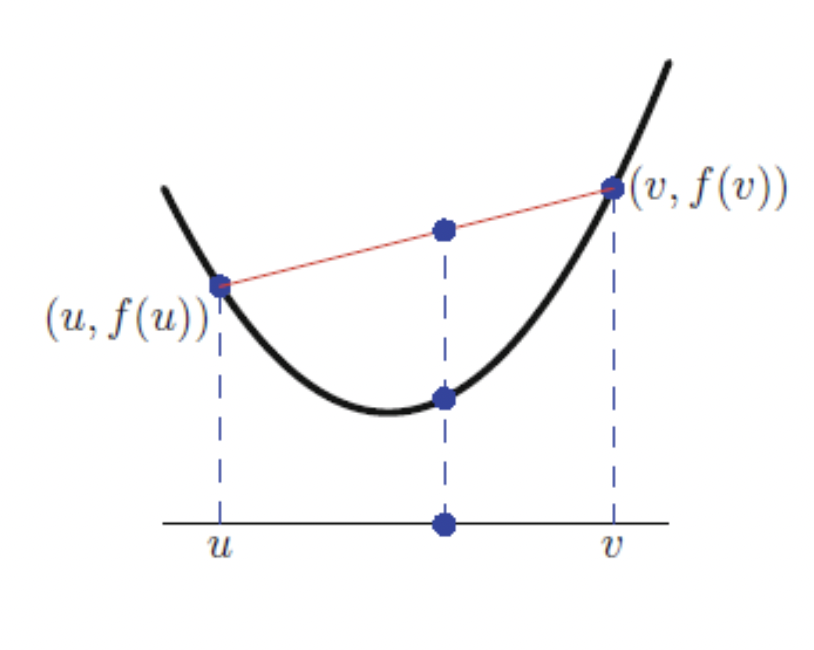
\includegraphics[width=0.5\textwidth]{fig1.1.png}
	\caption{Figura 1.1. Func\c{t}ii convexe: graficul este sub coarda}
\end{figure}

Aceast\u{a} remarc\u{a} arat\u{a} faptul ca func\c{t}iile convexe sunt majorate de func\c{t}iile afine pe orice subinterval compact.

Orice func\c{t}ie convex\u{a} f este marginit\u{a} pe fiecare subinterval compact \(\left [ u , v \right ]\) al intervalului pe care este definit\u{a}. De fapt , \(f\left ( x \right ) \leq  M = max \left \{ f\left ( u \right ), f\left ( v \right ) \right \}\)  pe \(\left [ u , v \right ]\)  \c{s}i scriind acest lucru \^{i}ntr-un punct arbitrar \(x\in  \left [ u , v  \right ]\)  de forma  \(x= \frac{\left ( u + v \right )}{2} + t\) pentru  \(t\) care verific\u{a} \(\left | t \right |\leq \frac{\left ( v - u \right )}{2}\), deducem cu usurin\c{t}\u{a} c\u{a}

\begin{displaymath}
  f\left ( x \right )=  f\left ( \frac{u+v}{2} + t\right )\geq 2 f\left ( \frac{u + v}{2} \right )- f\left ( \frac{u + v}{2} - t\right )\geq 2f\left ( \frac{u+v}{2} \right ) - M.
\end{displaymath}

\begin{theorem}
O func\c{t}ie convex\u{a} \(f: I \rightarrow \mathbb{R}\) este continu\u{a} \^{i}n orice punct interior al lui \(I\).   
\end{theorem}
\begin{proof}
  Presupunem c\u{a} \(a\in I\) \c{s}i alegem \(\varepsilon > 0\) astfel \^{i}ncat \(\left [ a - \varepsilon , a + \varepsilon  \right ] \subset I\).
 Atunci
\begin{displaymath}
  f\left ( a \right )\leq \frac{1}{2} f\left ( a - \varepsilon  \right ) + \frac{1}{2}f \left ( a + \varepsilon  \right )
\end{displaymath}
\c{s}i
\begin{displaymath}
  f\left ( a \pm t\varepsilon  \right )= f\left ( \left ( 1 - t \right ) a + t\left ( a \pm \varepsilon  \right )\right )\leq \left ( 1 - t \right )f\left ( a \right ) + tf\left ( a\pm \varepsilon  \right )
\end{displaymath}
pentru orice \(t\in \left [ 0 , 1 \right ]\). Prin urmare
\begin{displaymath}
  t\left ( f\left ( a\pm \varepsilon  \right ) - f\left ( a \right ) \right )\geq f\left ( a\pm t\varepsilon  \right )- f\left ( a \right )\geq -t\left ( f\left ( a\mp \varepsilon  \right ) - f\left ( a \right )\right )
\end{displaymath}
care ne conduce la
\begin{displaymath}
\left | f\left ( a\pm t\varepsilon  \right )- f\left ( a \right ) \right |\leq t max \left \{ \left | f\left ( a-\varepsilon  \right )- f\left ( a \right ) \right |, \left | f\left ( a+\varepsilon  \right ) - f\left ( a \right )\right | \right \},
\end{displaymath}
 pentru orice \(t\in \left [ 0 , 1 \right ]\). Continuitatea func\c{t}iei \(f\) este acum clar\u{a}.
 \end{proof}

 \begin{remark}
  Exemple simple precum, \(f\left ( x \right )= 0\) dac\u{a} \(x\in \left ( 0 , 1 \right )\), \c{s}i  \(f\left ( 0 \right )= f\left ( 1 \right ) = 1\), arat\u{a} faptul c\u{a} salturi  pot ap\u{a}rea \^{i}n capetele intervalului de defini\c{t}ie al unei func\c{t}ii convexe. Totu\c{s}i, aceste posibile discontinuit\u{a}\c{t}i pot fi \^{i}nl\u{a}turate.
\end{remark}


\begin{proposition}
Dac\u{a} \(f: \left [ a, b \right ]\rightarrow \mathbb{R}\) este o func\c{t}ie convex\u{a}, atunci limitele
\[
f\left ( a+ \right ) = \lim_{x\rightarrow a, x> a}f\left ( x \right ),~~ f\left ( b- \right ) = \lim_{x\rightarrow b, x< b}f\left ( x \right )\] exist\u{a} \^{i}n \(\mathbb{R}\) \c{s}i
\begin{displaymath}
  \tilde{f}\left ( x \right )= \left\{\begin{matrix}
f\left ( a+ \right ) & \\
 f\left ( x \right )& \\
 f\left ( b- \right )&
\end{matrix} \begin{matrix}
\text{dac\u{a} } x=a & \\
\text{dac\u{a} } x\in \left ( a,b \right ) & \\
\text{dac\u{a} } x= b&
\end{matrix}\right.
\end{displaymath}
 este o func\c{t}ie convex\u{a} continu\u{a}.
\end{proposition}
  Acest rezultat este o consecin\c{t}\u{a} a urm\u{a}toarelor rezultate :
\begin{lemma}

Dac\u{a} \(f: I \rightarrow \mathbb{R}\) este convex\u{a}, atunci sau \(f\) este monoton\u{a} pe intervalul \(I\), sau exist\u{a} un punct \(\xi \in int I\) astfel \^{i}ncat \(f\) este descresc\u{a}toare pe intervalul \(\left ( -\infty , \xi  \right )\cap I\) \c{s}i cresc\u{a}toare pe intervalul \(\left[\xi , \infty  \right )\cap I\).
\end{lemma}
\begin{proof}
Lu\u{a}m \(a < b\) puncte interioare arbitrare ale lui \(I\) \c{s}i fie
\[m = inf\left \{ f\left ( x \right ): ~~x\in \left [ a,b \right ]\right \}.\] Cum \(f\) este continu\u{a} pe \(\left [ a,b \right ]\), acest infimum este atins \^{i}n punctul \(\xi \in \left [ a,b \right ]\), adic\u{a}
$
  m = f\left ( \xi  \right )
$
Dac\u{a} \(a \leq x <  y< \xi\), atunci \(y\) este o combina\c{t}ie convex\u{a} a lui \(x\) \c{s}i \(\xi\), mai exact, \[y = \frac{\xi -y}{\xi -x}x + \frac{y - x}{\xi -x}\xi.\] Cum \(f\) este convex\u{a},
\begin{displaymath}
  f\left ( y \right )\leq \frac{\xi -y}{\xi -x}f\left ( x \right )+ \frac{y-x}{\xi -x}f\left ( \xi  \right )\leq f\left ( x \right ).
\end{displaymath}
Demonstra\c{t}ia se \^{i}ncheie cu un proces de lipire (la stanga lui \(a\) \c{s}i la dreapta lui \(b\)), observ\^{a}nd c\u{a} proprietatea de covexitate face imposibil\u{a} existen\c{t}a a trei numere \(u < v < w\) \^{i}n \(I\) astfel \^{i}nc\^{a}t \(f\left ( u \right ) < f\left ( v \right )> f\left ( w \right )\).
\end{proof}

\begin{corollary}
\begin{enumerate}[a)]
\item Orice func\c{t}ie convex\u{a} \(f: I \rightarrow \mathbb{R}\) care nu este monoton\u{a} pe
intervalul \(I\) are un minim global interior.
\item Dac\u{a} o func\c{t}ie convex\u{a} \(f: \mathbb{R} \rightarrow \mathbb{R}\) este marginit\u{a} superior, atunci este constant\u{a}.
\end{enumerate}
\end{corollary}
Atingere supremului la capete nu este o proprietate caracteristic\u{a} a func\c{t}iilor convexe, dar vom avea \^{i}ns\u{a} urmatorul rezultat.

\begin{theorem}

Fie \(f: I \rightarrow \mathbb{R}\). Atunci \(f\) este (strict) convex\u{a} daca \c{s}i numai dac\u{a} pentru orice subinterval compact \(J\) al lui \(I\), \c{s}i fiecare func\c{t}ie afin\u{a} \(L\), supremul lui \(f+L\) pe \(J\) este atins \^{i}ntr-un cap\u{a}t al intervalului (\c{s}i doar acolo).
\end{theorem}

\begin{proof}
Ne vom restrange la cazul func\c{t}iilor convexe. Cazul func\c{t}iilor strict convexe poate fi tratat \^{i}n acelasi mod.

\textbf{Necesitatea:} Dac\u{a} \(f\) este convex\u{a}, la fel este \c{s}i suma \(F = f + L\). Cum orice punct al unui subinterval \(J = \left [ x , y \right ]\) este o combina\c{t}ie convex\u{a} \(z = \left ( 1 - \lambda  \right )x + \lambda y \) a lui \(x\) \c{s}i \(y\), avem
\begin{equation*}
\begin{split}
  \sup_{z\in J}F\left ( z \right ) &= \sup_{\lambda \in \left [ 0 , 1 \right ]}F\left ( \left ( 1 - \lambda  \right )x + \lambda y \right )\\
  &\leq \sup_{\lambda \in \left [ 0,1 \right ]}\left [ \left ( 1-\lambda  \right )F\left ( x \right ) + \lambda F\left ( y \right ) \right ] + max \left \{ F\left ( x \right ), F\left ( y \right ) \right \}
  \end{split}
\end{equation*}

\textbf{Suficien\c{t}a:} Av\^{a}nd un subinterval \(J = \left [ x,y \right ]\) al lui \(I\), exist\u{a} o func\c{t}ie afin\u{a} \(L\left ( x \right ) = mx + n\) care este egal\u{a} cu \(f\) \^{i}n cele doua puncte  \(x\) si \(y\).
Atunci
\begin{displaymath}
  \sup_{\lambda \in \left [ 0,1 \right ]}\left [ \left ( f - L \right )\left ( 1 - \lambda  \right )x + \lambda y \right ] = 0,
\end{displaymath}
care ne conduce la
\begin{displaymath}
  0\geq f\left ( \left ( 1 - \lambda  \right )x + \lambda y \right )- L\left ( \left ( 1 - \lambda  \right )x - \lambda L \right )
\end{displaymath}
  \begin{displaymath}
  = f\left ( \left ( 1 - \lambda  \right )x + \lambda y  \right ) - \left ( 1 - \lambda  \right )L\left ( x \right ) - \lambda L\left ( y \right )
\end{displaymath}
\begin{displaymath}
  = f\left ( \left ( 1 - \lambda  \right )x + \lambda y \right ) - \left ( 1 - \lambda  \right ) f\left ( x \right ) - \lambda f \left ( y \right ),
\end{displaymath}
pentru orice \(\lambda \in \left [ 0,1 \right ]\).
\end{proof}

\begin{definition}
O func\c{t}ie \(f: I \rightarrow \mathbb{R}\) se nume\c{s}te cvasiconvex\u{a} dac\u{a},
 \begin{displaymath}
  f\left ( \left ( 1-\lambda  \right )x + \lambda y \right )\geq  min\left \{ f\left ( x \right ), f\left ( y \right ) \right \}
\end{displaymath}
pentru orice  \(x, y \in I\) \c{s}i \(\lambda  \in \left ( 0,1 \right ]\).
\end{definition}
   Avem urm\u{a}toarea caracterizare a convexit\u{a}\c{t}ii \^{i}n cadrul clasei func\c{t}iilor continue care se dovede\c{s}te util\u{a} \c{s}i \^{i}n verificarea convexit\u{a}\c{t}ii.
\begin{theorem}
O func\c{t}ie \(f : I \rightarrow \mathbb{R}\) este convex\u{a} dac\u{a} \c{s}i numai dac\u{a} ea verific\u{a} urmatoarele dou\u{a} condi\c{t}ii:
\begin{enumerate}[a)]
\item \(f\) este continu\u{a} \^{i}n fiecare punct din interiorul lui \(I\); \c{s}i
\item \(f\) este convex\u{a} \^{i}n punctul de mijloc , adic\u{a},
\end{enumerate}
\begin{displaymath}
  f\left ( \frac{x+y}{2} \right )\leq \frac{f\left ( x \right )+f\left ( y \right )}{2}, \text{ pentru orice } x, y \in I.
\end{displaymath}
\end{theorem}
\begin{proof}
\textbf{Necesitatea }rezult\u{a} din teorema 1.

\textbf{Suficien\c{t}a} o vom demonstra prin reducere la absurd. Dac\u{a} \(f\) nu este convex\u{a}, atunci exist\u{a} un interval \(\left [ a,b \right ]\) astfel \^{i}nc\^{i}t graficul func\c{t}iei \(f\) restric\c{t}ionat\u{a} la  \(\left [ a,b \right ]\) s\u{a} nu fie sub coarda care une\c{s}te punctele \(\left ( a, f\left ( a \right ) \right )\) \c{s}i \(\left ( b, f\left ( b \right ) \right )\); ca urmare , func\c{t}ia
\begin{displaymath}
  \varphi \left ( x \right )= -f\left ( x \right ) + f\left ( a \right )+ \frac{f\left ( b \right )- f\left ( a \right )}{b-a}\left ( x-a \right ), x\in \left [ a,b \right ]
\end{displaymath}
are  \(\gamma = \inf \left \{ \varphi \left ( x \right ) : x\in \left [ a,b \right ]\right \}< 0\).

Observam c\u{a} \(-\varphi\) este convex\u{a} \^{i}n punctul de mijloc, continu\u{a} \c{s}i \(\varphi \left ( a \right ) =\varphi \left ( b \right ) = 0\). Fie \(c = inf \left \{ x \in \left [ a,b  \right ] : \varphi \left ( x \right )= \gamma \right \} \), atunci \(\varphi \left ( c \right ) = \gamma\)  \c{s}i \(c \in \left ( a,b  \right )\). Conform defini\c{t}iei lui \(c\), pentru orice \(h>0\), pentru care \(c\pm h\in \left ( a,b \right )\), avem
\begin{displaymath}
  \varphi \left ( c - h  \right )> \varphi \left ( c \right ) si \varphi \left ( c + h  \right )\geq  \varphi \left ( c \right )
\end{displaymath}

\noindent Astfel
\begin{displaymath}
  -\varphi \left ( c \right )> \frac{-\varphi \left ( c-h \right )-\varphi \left ( c+h \right )}{2},
\end{displaymath}
ceea ce este \^{i}n contradic\c{t}ie cu faptul c\u{a} \(-\varphi\) este convex\u{a} \^{i}n punctul de mijloc.
\end{proof}


\begin{corollary}
Fie \(f: I \rightarrow \mathbb{R}\) o func\c{t}ie continu\u{a}. Atunci, \(f\) este convex\u{a} dac\u{a} \c{s}i numai dac\u{a}
\begin{displaymath}
  f\left ( x+h \right )+ f\left ( x - h \right ) - 2f\left ( x \right )\geq 0
\end{displaymath}
pentru orice \(x \in I\) \c{s}i orice \(h > 0\) astfel \^{i}nc\^{a}t \c{s}i \(x + h\) \c{s}i \(x - h\) apar\c{t}in lui \(I\).
\end{corollary}
\begin{remark}
Observ\u{a}m c\u{a} \c{s}i eorema 3 \c{s}i corolarul 2 de mai sus, admit variante \^{i}n cazul func\c{t}iilor strict convexe,
Corolarul 2 ne permite s\u{a} verific\u{a}m imediat convexitatea / concavitatea strict\u{a} a unor func\c{t}ii elementare, precum func\c{t}ia exponen\c{t}ial\u{a}, cea logaritmic\u{a}, \c{s}i restric\c{t}ia func\c{t}iei sinus pe \(\left [ 0 , \pi \right ]\).

\^{I}ntr-adevar, pentru func\c{t}ia exponen\c{t}ial\u{a}, faptul c\u{a}  \(a , b > 0, a\neq b\), implic\u{a} \(\frac{a + b}{2}> \sqrt{ab}\)
este echivalent\u{a} cu
\(e^{x + h} + e^{x - h } - 2e^{x}> 0\)
pentru orice \(x\in \mathbb{R}\) \c{s}i orice \(h > 0\).
\end{remark}
  Multe alte exemple pot fi deduse folosind urm\u{a}toarele propriet\u{a}\c{t}i ale func\c{t}iilor convexe / concave.

\begin{proposition}
\textbf{Opera\c{t}ii cu func\c{t}ii convexe:}
\begin{enumerate}[a)]
\item Adun\^{a}nd dou\u{a} func\c{t}ii convexe ( definite pe acela\c{s}i interval) ob\c{t}inem o func\c{t}ie convex\u{a}; dac\u{a} una dintre ele este strict convex\u{a}, atunci suma lor este de asemenea strict convex\u{a}.
\item \^{I}nmul\c{t}ind o func\c{t}ie (strict) convex\u{a} cu un scalar (strict)  pozitiv ob\c{t}inem de asemenea o func\c{t}ie (strict) convex\u{a}.
\item Presupunem c\u{a} f \c{s}i g sunt dou\u{a} func\c{t}ii convexe pozitive definite pe un interval I. Atunci, produsul lor este o func\c{t}ie convex\u{a} pe I dac\u{a} sunt sincrone \^{i}n sensul c\u{a}, \begin{displaymath}
   \left ( f\left ( x \right ) - f\left ( y \right ) \right )\left ( g\left ( x \right ) - g\left ( y \right )\right )\geq 0
\end{displaymath} pentru orice \(x , y \in \mathbb{R}\); de exemplu , aceast\u{a} condi\c{t}ie apare daca f \c{s}i g sunt amandou\u{a} descresc\u{a}toare sau am\^{a}ndou\u{a} cresc\u{a}toare.
\item Restric\c{t}ia unei func\c{t}ii (strict) convexe pe I, la un subinterval al lui I este de asemenea o func\c{t}ie (strict) convex\u{a}.
\item Presupunem c\u{a} \(f\) este o func\c{t}ie bijectiv\u{a} \^{i}ntre dou\u{a} intervale \(I\) si \(J\). Dac\u{a} \(f\) este strict cresc\u{a}toare, atunci \(f\) este (strict) convex\u{a} dac\u{a} \c{s}i numai dac\u{a} \(f^{-1}\) este (strict) concav\u{a}. Dac\u{a} \(f\) este o func\c{t}ie bijectiv\u{a} descresc\u{a}toare, atunci \(f\) \c{s}i  \(f^{-1}\) sunt ambele convexe sau ambele concave.
\item Dac\u{a} \(f\) este o func\c{t}ie strict pozitiv\u{a} concav\u{a}, atunci \(\frac{1}{f}\) este o func\c{t}ie convex\u{a}. Aici rolul concavit\u{a}\c{t}ii \c{s}i al convexit\u{a}\c{t}ii nu poate fi schimbat unul cu cel\u{a}lalt.
\item Maximul a dou\u{a} func\c{t}ii (stricte) convexe \(f , g : I \rightarrow \mathbb{R}\),
\begin{displaymath}
  max \left \{ f , g \right \}\left ( x \right )=  max \left \{ f\left ( x \right ), g\left ( x \right ) \right \}
\end{displaymath} este de asemenea o func\c{t}ie (strict) convex\u{a}.
\item Compunerea \(f\left ( ax + b \right )\), a unei func\c{t}ii \(f\) convexe \c{s}i a unei func\c{t}ii afine \(ax+b\), este o func\c{t}ie convex\u{a}.
\end{enumerate}
\end{proposition}
\^{I}n continuare, vom discuta extinderea inegalit\u{a}\c{t}ii convexit\u{a}\c{t}ii 1.1. \^{I}n primul r\^{a}nd, observ\u{a}m faptul c\u{a} intervalele sunt \^{i}nchise la combina\c{t}ii convexe arbitrare, adic\u{a},
\begin{displaymath}
  \sum_{ k= 1}^{n}\lambda _{k}x_{k} \in I~~\mbox{pentru orice}~~x_{1},\cdots, x_{n} \in I  ~~\mbox{\c{s}i orice}~~\lambda _{1},\cdots, \lambda _{n} \in \left [ 0 , 1  \right ]
\end{displaymath}
 cu \(\sum_{k = 1}^{n} \lambda _{k} = 1\).
Acest lucru poate fi demonstrat prin induc\c{t}ie dup\u{a} \(n\).

\noindent Cazul \(n=1\) este trivial, \^{i}n timp ce \(n = 2\) rezult\u{a} din defini\c{t}ia unei mul\c{t}imi convexe.

  Presupun\^{a}nd faptul c\u{a} rezultatul este adev\u{a}rat pentru toate combina\c{t}iile convexe cu cel mult \(n\geq 2\) puncte, s\u{a} trecem la cazul combina\c{t}iilor cu \(n + 1\) puncte, \(x = \sum_{k = 1}^{n + 1} \lambda _{k}x_{k}\). Cazul non-trivial este atunci c\^{a}nd to\c{t}i coeficien\c{t}ii \(\lambda _{k}\) se afl\u{a} \^{i}n \(\left ( 0 , 1 \right )\). Dar \^{i}n acest caz, datorit\u{a} ipotezei de induc\c{t}ie, x poate fi reprezentat ca o combina\c{t}ie convex\u{a} de dou\u{a} elemente ale lui \(I\),
\begin{displaymath}
  x = \left ( 1 - \lambda _{n + 1} \right )\left ( \sum_{k = 1}^{n} \frac{\lambda _{k}}{1 - \lambda _{n + 1}} x_{k}\right ) + \lambda _{n + 1}x_{n + 1},
\end{displaymath}
prin urmare x apar\c{t}ine lui \(I\).
  Observa\c{t}ia de mai sus asupra intervalelor are o echivalen\c{t}\u{a} remarcabil\u{a} pentru func\c{t}iile convexe:

\begin{lemma}
\textbf{Cazul discret al inegalit\u{a}\c{t}ii lui Jensen}

O func\c{t}ie cu valori reale \(f\) definit\u{a} pe un interval \(I\) este convex\u{a} dac\u{a} \c{s}i numai dac\u{a} pentru orice puncte \(x_{1},\cdots,x_{n}\) din \(I\) \c{s}i orice scalari \(\lambda _{1},\cdots,\lambda _{n}\) din \(\left [ 0 , 1 \right ]\) cu \(\sum_{k = 1}^{n}\lambda _{k}= 1\) avem,
\begin{displaymath}
  f\left ( \sum_{k = 1}^{n} \lambda _{k}x_{k}\right )\leq \sum_{k = 1}^{n}\lambda _{k}f\left ( x_{k} \right ).
\end{displaymath}

Dac\u{a} \(f\) este strict convex\u{a}, inegalitatea de mai sus este strict\u{a} dac\u{a} punctele \(x_{k}\) nu sunt toate egale \^{i}ntre ele , \c{s}i scalarii \(\lambda _{k}\) sunt to\c{t}i pozitivi.
\end{lemma}
\begin{proof}
Prima afirma\c{t}ie rezult\u{a} prin induc\c{t}ie matematic\u{a}.

\^{I}n ceea ce prive\c{s}te cea de a doua afirma\c{t}ie, presupunem c\u{a} func\c{t}ia \(f\) este strict convex\u{a} \c{s}i
\begin{displaymath}
  f\left ( \sum_{k = 1}^{n} \lambda _{k}x_{k}\right )=  \sum_{k = 1}^{n}\lambda _{k}f\left ( x_{k} \right ). \label{eq:1.3} \tag{1.3}
\end{displaymath}
pentru  punctele \(x_{1}, \cdots, x_{n} \in I\) \c{s}i scalarii \(\lambda _{1}, \cdots, \lambda _{n} \in \left ( 0 , 1\right )\) care au suma egal\u{a}  cu \(1\). Dac\u{a} \(x_{1}, \cdots, x_{n}\) nu sunt to\c{t}i egali, mul\c{t}imea
\[S = \left \{ k: x_{k}<  max \left \{ x_{1,\cdots,x_{n}} \right \} \right \}\]
 va fi o submul\c{t}ime proprie a mul\c{t}imii  \(\left \{ 1,\cdots,n \right \}\) \c{s}i \(\lambda _{S} = \sum_{k \in S}^{}\lambda _{S} \in \left ( 0,1 \right )\). Cum \(f\) este strict convex\u{a} avem,
 \begin{equation} \nonumber
     \begin{split}
         f\left ( \sum_{k=1}^{n}\lambda _{k}x_{k} \right ) & = f\left ( \lambda _{S}\left ( \sum_{k\in S}^{}\frac{\lambda _{k}}{\lambda _{S}} x_{k}\right ) +\left ( 1-\lambda _{S} \right )\left ( \sum_{k\notin S}^{} \frac{\lambda _{k}}{1 - \lambda _{S}}x_{k}\right )\right ) \\ & <\lambda _{S}f\left ( \sum_{k\in S}^{}\frac{\lambda _{k}}{\lambda _{S}} x_{k}\right ) +\left ( 1 - \lambda _{S} \right )f\left ( \sum_{k\notin S}^{}\frac{\lambda _{k}}{1 - \lambda _{S}} x_{k}\right ) \\ & <\lambda _{S} \sum_{k\in S}^{}\frac{\lambda _{k}}{\lambda _{S}} f\left ( x_{k} \right ) +\left ( 1 - \lambda _{S} \right ) \sum_{k\notin S}^{}\frac{\lambda _{k}}{1 - \lambda _{S}}f\left ( x_{k} \right ) \\ & = \sum_{k=1}^{n}\lambda _{k}f\left ( x_{k} \right ),
     \end{split}
 \end{equation}
care contrazice ipoteza noastr\u{a} \ref{eq:1.3}. Astfel, toate punctele \(x_{k}\) ar trebui s\u{a} coincid\u{a}.
\end{proof}

O consecin\c{t}\u{a} imediat\u{a} a lemei 2 (c\^{a}nd este aplicat\u{a} func\c{t}iei exponen\c{t}iale) este urm\u{a}torul rezultat care extinde bine cunoscuta inegalitate MA-MG (adic\u{a} inegalitatea dintre media aritmetic\u{a} \c{s}i cea geometric\u{a}).


\begin{theorem}
\textbf{Forma ponderat\u{a} a inegali\u{a}\c{t}ii mediilor}

Dac\u{a} \(x_{1},\cdots,x_{n}\in \left ( 0,\infty  \right ) si \lambda_{1},\cdots,\lambda _{n} \in \left ( 0 , 1 \right ), \sum_{k = 1}^{n}\lambda _{k}= 1\), atunci
\begin{displaymath}
  \sum_{k = 1}^{n}\lambda _{k}x_{k}> x_{1}^{\lambda _{1}}\cdots x_{n}^{\lambda _{n}}
\end{displaymath}
\^{i}n afar\u{a} de cazul c\^{a}nd \(x_{1} = \cdots = x_{n}\).
  
  \^{I}nlocuind \(x_{k}\) cu \(\frac{1}{x_{k} }\) \^{i}n ultima inegalitate, ob\c{t}inem
\begin{displaymath}
  x_{1}^{\lambda _{1}}\cdots x_{n}^{\lambda _{n}}> \frac{1}{\sum_{k = 1}^{n}\lambda _{k}\frac{1}{x_{k}}}
\end{displaymath}
\^{i}n afar\u{a} de cazul c\^{a}nd \(x_{1} = \cdots = x_{n}\).
\end{theorem}
Aceasta reprezint\u{a} forma ponderat\u{a} a inegalit\u{a}\c{t}ii mediei geometrice – mediei armonice (adic\u{a} inegalitatea MG-MH).

Pentru \(\lambda _{1} = \cdots =\lambda _{n}= \frac{1}{n}\) ob\c{t}inem inegalitatea obi\c{s}nuit\u{a} care afirm\u{a} c\u{a} pentru orice \(x_{1},\cdots,x_{n}\)  numere pozitive, nu toate egale, avem

\begin{displaymath}
  \frac{x_{1}+\cdots+x_{n}}{n}> \sqrt[n]{x_{1}\cdots x_{n}}> \frac{n}{\left ( \frac{1}{x_{1}}+\cdots+\frac{1}{x_{n}} \right )}.
\end{displaymath}




\section{Inegalitatea lui Young \c{s}i consecin\c{t}ele sale}

Urm\u{a}torul caz special al formei ponderate a inegalit\u{a}\c{t}ii MA-MG este cunoscut sub numele de inegalitatea lui Young:
\begin{displaymath}
  ab \leq \frac{a^{p}}{p}+ \frac{b^{q}}{q}, \label{eq: 1.4} \tag{1.4}
\end{displaymath}
pentru orice \(a,b \geq 0\)
\c{s}i pentru orice  \(p,q \in \left ( 0 , 1 \right )\) cu proprietatea c\u{a} \(\frac{1}{p}+\frac{1}{q} = 1\).
Egalitatea are loc dac\u{a} \c{s}i numai dac\u{a} \(a^{p}= b^{q}\).

Inegalitatea lui Young poate fi de asemenea ob\c{t}inut\u{a} ca o consecin\u{a} a convexit\u{a}\c{t}ii stricte a func\c{t}iei exponen\c{t}iale.

\^{I}ntr-adevar
\begin{equation} \nonumber
    \begin{split}
        ab & =  e^{\log_{a}b} \\ & = e^{\left (\frac{1}{p}  \right )\log_{a}p+ \left ( \frac{1}{q} \right )\log_{b}q} \\ & < \frac{1}{p}e^{\log_{a}p}+\frac{1}{q}e^{\log_{b}q} \\ & = \frac{a^{p}}{p}+\frac{b^{q}}{q},
    \end{split}
\end{equation}
pentru orice \(a,b>0\) astfel \^{i}nc\^{a}t \(a^{p}\neq b^{q}\).

O alt\u{a} solu\c{t}ie este oferit\u{a} de studiul varia\c{t}iei func\c{t}iei diferen\c{t}iabile
\begin{displaymath}
  F\left ( a \right )= \frac{a^{p}}{p}+\frac{b^{q}}{q} - ab,~ a\geq 0,
\end{displaymath}
unde \(b\geq 0\) este un paramentru. Aceast\u{a} func\c{t}ie \^{i}\c{s}i atinge punctul de minim global strict \^{i}n \(a= b^{\frac{q}{p}}\), care ne conduce la \(F\left ( a \right )> F\left ( b^{\frac{q}{p}} \right ) = 0\) pentru orice \(a\geq 0, a\neq b^{\frac{q}{p}}\).

  W.H.Young a dovedid de fapt  o inegalitate mult mai general\u{a}, pentru \(f\left ( x \right )=  x^{p-1}\).

\begin{theorem}
\textbf{Inegalitatea lui Young
}
Presupunem c\u{a} \(f: \left [ 0,\infty  \right ) \rightarrow \left [ 0,\infty  \right )\) este o func\c{t}ie continu\u{a} strict cresc\u{a}toare astfel \^{i}nc\^{a}t \(f\left ( 0 \right )= 0\) \c{s}i \(\lim_{x\rightarrow \infty }f\left ( x \right )= \infty\). Atunci
\begin{displaymath}
  uv\leq \int_{0}^{u}f\left ( x \right )dx + \int_{0}^{v}f^{-1}\left ( y \right )dy
\end{displaymath}
pentru orice \(u,v\geq 0\) cu egalitate dac\u{a} \c{s}i numai dac\u{a} \( v = f\left ( u \right )\).
\end{theorem}

\begin{figure}[htbp]
	\centering
	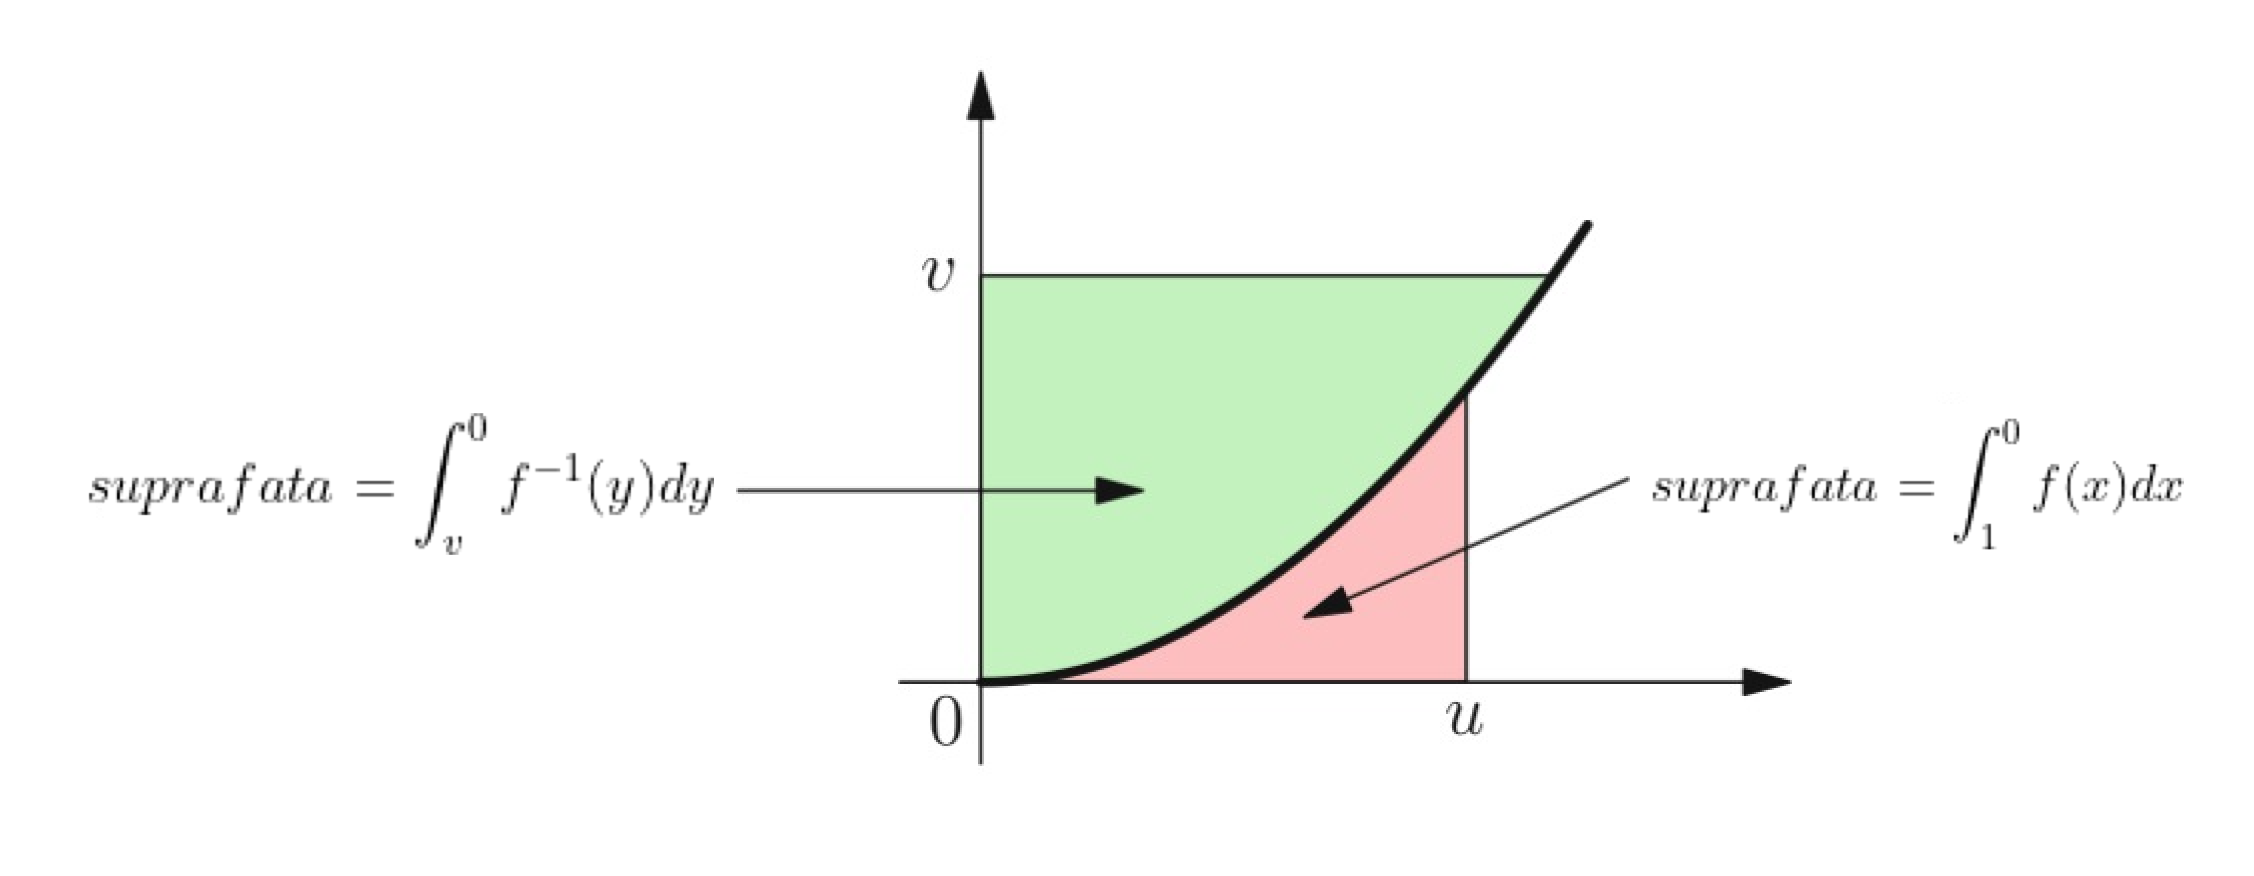
\includegraphics[width=1.0\textwidth]{fig1.2.png}
	\caption{Figura 1.2. Aria  de unire a celor doua triunghiuri curbilinii dep\u{a}\c{s}e\c{s}te aria dreptunghiului cu laturile u \c{s}i v}
\end{figure}

\begin{proof}
Folosind defini\c{t}ia derivatei se poate demonstra cu usurin\c{t}\u{a} c\u{a} func\c{t}ia
\begin{displaymath}
  F\left ( u \right )= \int_{0}^{u}f\left ( x \right )dx + \int_{0}^{f\left ( u \right )}f^{-1}\left ( y \right )dy -uf\left ( u \right ), u \in \left [ 0,\infty  \right )
\end{displaymath}
este diferen\c{t}iabil\u{a}, cu \({F}'\) $\equiv 0.$ Astfel, \(F\left ( u \right )= F\left ( 0 \right )= 0\) pentru orice \(u\geq 0\).
  
Dac\u{a} \(u, v \geq 0\)  \c{s}i \(v\geq f\left ( u \right )\), atunci
\begin{equation} \nonumber
    \begin{split}
       uv & =  uf\left ( u \right )+ u\left ( v- f\left ( u \right ) \right ) \\ &  =  \int_{0}^{u}f\left ( x \right )dx + \int_{0}^{f\left ( u \right )}f^{-1}\left ( y \right )dy + u\left ( v - f\left ( u \right ) \right ) \\ &  = \int_{0}^{u}f\left ( x \right )dx + \int_{0}^{v}f^{-1}\left ( y \right )dy + \left [ u\left ( v-f\left ( u \right )  \right ) - \int_{f\left ( u \right )}^{v}f^{-1}\left ( y \right )dy\right ] \\ &  \leq \int_{0}^{u}f\left ( x \right )dx + \int_{0}^{v}f^{-1}\left ( y \right )dy.
    \end{split}
\end{equation}
Cel\u{a}lalt caz, unde \(v\leq f\left ( u \right )\) poate fi tratat similar.
\end{proof}

\begin{theorem}

\textbf{Inegalitatea lui Rogers-Hölder pentru} \(p > 1\)

Fie \(p,q \in \left ( 1, \infty  \right )\) cu \(\frac{1}{p} + \frac{1}{q} = 1\) \c{s}i  \(f\in L^{p}\left ( \mu  \right )\) si \(g\in L^{q}\left ( \mu  \right )\). Atunci \(fg\) apar\c{t}ine lui \(L^{1}\left ( \mu  \right )\) \c{s}i avem
\begin{displaymath}
  \left | \int_{\Omega}^{} fg  d\mu \right |\leq \int_{\Omega}^{}\left | fg \right |d\mu \label{eq:1.5} \tag{1.5}
\end{displaymath}
\c{s}i
\begin{displaymath}
  \int_{\Omega}^{}\left | fg \right |d\mu \leq \left \| f \right \|_{L^{p}}\left \| g \right \|_{{L}^{q}}. \label{eq:1.6} \tag{1.6}
\end{displaymath}
Ca o consecin\c{t}\u{a}
\begin{displaymath}
  \left | \int_{\Omega}^{} fg  d\mu \right |\leq \left \| f \right \|_{L^{p}}\left \| g \right \|_{{L}^{q}}. \label{eq:1.7} \tag{1.7}
\end{displaymath}
\end{theorem}

\begin{remark}
  Rezultatul de mai sus se extinde \^{i}ntr-o manier\u{a} direct\u{a} la perechi de forma \(p = 1, q = \infty\) \c{s}i \(p = \infty, q = 1\).
  
Din Inegalitatea Rogers – Hölder rezult\u{a} c\u{a} pentru orice \(p, q, r \in \left ( 1 , \infty  \right )\) cu \(\frac{1}{p} + \frac{1}{q} = 1\) \c{s}i orice \(f\in L^{p}\left ( \mu  \right )\) si \(g\in L^{q}\left ( \mu  \right )\) avem \(fg\in L^{r}\left ( \mu  \right )\) \c{s}i
\begin{displaymath}
  \left \| fg \right \|_{L^{r}}\leq \left \| f \right \|_{L^{p}}\left \| g \right \|_{L^{q}} \label{eq:1.8} \tag{1.8}
\end{displaymath}


Inegalitatea \ref{eq:1.8}, pentru \(p = q = 2\), este cunoscut\u{a} ca \textbf{inegalitatea Cauchy-Bunyakovsky-Schwarz} pentru integrale.
\end{remark}
\begin{proof}
Prima inegalitate este trivial\u{a}.

Dac\u{a} \(f\) sau \(g\) sunt \(0~~ \mu\) – aproape peste tot, atunci cea de a doua inegalitate este trivial\u{a}. Altfel, folosind inegalitatea lui Young, avem
\begin{displaymath}
  \frac{\left | f\left ( x \right ) \right |}{\left \| f \right \|_{L^{p}}} \cdot \frac{\left | g\left ( x \right ) \right |}{\left \| g \right \|_{L^{q}}}\leq \frac{1}{p}\cdot \frac{\left | f\left ( x \right ) \right |^{p}}{\left \| f \right \|^{p}_{L^{p}}} + \frac{1}{q}\cdot \frac{\left | g\left ( x \right ) \right |^{q}}{\left \| g \right \|^{q}_{L^{q}}}
\end{displaymath}
 pentru orice \(x\) din \(\Omega\). Astfel deducem c\u{a} \(fg \in L^{1}\left ( \mu  \right )\). De asemenea
\begin{displaymath}
  \frac{1}{\left \| f \right \|_{L^{p}}\left \| g \right \|_{L^{q}}}\int_{\Omega }\left | fg \right |d\mu \leq 1.
\end{displaymath}
\end{proof}

\begin{remark}

Condi\c{t}ii pentru egalitatea din teorma 6

Observa\c{t}ia de baz\u{a} este faptul c\u{a}  \(f\geq 0\) \c{s}i \(\int_{\Omega }f d\mu  = 0\) implic\u{a} \(f = 0~~ \mu-\) aproape peste tot.
  Prin urmare avem egalitate \^{i}n \ref{eq:1.6} dac\u{a} \c{s}i numai dac\u{a}
\begin{displaymath}
  f\left ( x \right )g\left ( x \right ) = e^{i\theta }\left | f\left ( x \right ) g\left ( x \right )\right |
\end{displaymath}
pentru o constant\u{a} real\u{a} \(\theta\) \c{s}i pentru \(\mu-\) aproape peste to\c{t}i \(x\).


  Presupunem c\u{a} \(p , q \in \left ( 1 , \infty  \right )\) \c{s}i \(f\) si \(g\) nu sunt zero \(\mu-\) aproape peste tot. Pentru a avea egalitate \^{i}n \ref{eq:1.6} este necesar \c{s}i suficient s\u{a} avem
\begin{displaymath}
  \frac{\left | f\left ( x \right ) \right |}{\left \| f \right \|_{L^{p}}} \cdot \frac{\left | g\left ( x \right ) \right |}{\left \| g \right \|_{L^{q}}}\leq \frac{1}{p}\cdot \frac{\left | f\left ( x \right ) \right |^{p}}{\left \| f \right \|^{p}_{L^{p}}} + \frac{1}{q}\cdot \frac{\left | g\left ( x \right ) \right |^{q}}{\left \| g \right \|^{q}_{L^{q}}}
\end{displaymath}
\(\mu-~\)aproape peste tot.

\noindent Cazul egalit\u{a}\c{t}ii \^{i}n Inegalitatea lui Young demonstreaz\u{a} c\u{a} aceasta este echivalent\u{a} cu \(A\left | f\left ( x \right ) \right |^{p} = B\left | g\left ( x \right ) \right |^{q}~~ \mu-\)aproape peste tot,
unde A \c{s}i B sunt dou\u{a} constante pozitive.

  Dac\u{a} \(p = 1\) si \(q = \infty\), avem egalitate \^{i}n ecua\c{t}ia \ref{eq:1.6} dac\u{a} \c{s}i numai dac\u{a} exist\u{a} o constant\u{a} \(\lambda \geq 0\) astfel \^{i}nc\^{a}t \(\left | g\left ( x \right ) \right |\leq \lambda\),  \(\mu\) aproape peste tot \c{s}i \(\left | g\left ( x \right ) \right |= \lambda,  \mu\) aproape peste tot pe mul\c{t}imea \(\left \{ x : f\left ( x \right )\neq 0 \right \}\).
\end{remark}
\begin{theorem}
\textbf{Inegalitatea Minkowski}\\

Pentru \(1\leq  p < \infty\) \c{s}i \(f , g \in L^{p}\left ( \mu  \right ) \) avem
\begin{displaymath}
  \left \| f + g  \right \|_{L^{p}}\leq \left \| f \right \|_{L^{p}} + \left \| g \right \|_{L^{p}}. \label{eq:1.9} \tag{1.9}
\end{displaymath}
\end{theorem}
\begin{proof}
Pentru \(p  = 1\), inegalitatea \ref{eq:1.9} rezult\u{a} imediat prin integrarea inegalit\u{a}\c{t}ii \(\left | f + g \right |\leq \left | f \right | + \left | g \right |\). Pentru \(p \in \left ( 1 , \infty  \right )\) avem:
\begin{equation} \nonumber
    \begin{split}
        \left | f + g  \right |^{p} &   \leq \left ( \left | f \right | +\left | g \right |\right )^{p} \\ & \leq \left ( 2 \sup\left \{ \left | f \right |,\left | g \right | \right \} \right )^{p} \\ & \leq 2^{p}\left ( \left | f \right |^{p}  + \left | g \right |^{p}\right )
    \end{split}
\end{equation}
care ne demonstreaz\u{a} c\u{a} \(f + g \in L^{p}\left ( \mu  \right )\). Mai mult de at\^{a}t, conform teoremei 6,
\begin{equation} \nonumber
    \begin{split}
         \left \| f + g  \right \|_{L^{p}}^{p}  &  = \int_{\Omega }\left | f + g \right |^{p}d\mu \\ & \leq \int_{\Omega }\left | f + g \right |^{p - 1}\left | f \right |d\mu + \int_{\Omega }\left | f + g  \right |^{p - 1}\left | g \right |d\mu \\ & \leq\left ( \int_{\Omega }\left | f \right |^{p}d\mu  \right )^{\frac{1}{p}}\left ( \int_{\Omega }\left | f + g  \right | ^{\left ( p - 1 \right )}d\mu \right )^{\frac{1}{q}}+ \left ( \int_{\Omega }\left | g \right |^{p}d\mu  \right )^{\frac{1}{p}}\left ( \int_{\Omega} \left | f + g \right |^{\left ( p - 1 \right )q}d\mu \right )^{\frac{1}{q}} \\ &  =\left ( \left \| f \right \|_{L^{p}} + \left \| g \right \|_{L^{p}} \right )\left \| f + g  \right \|_{L^{p}}^{\frac{p}{q}}
    \end{split}
\end{equation}
unde \(\frac{1}{p} + \frac{1}{q} = 1\), deci avem c\u{a} \(p - \frac{p}{q} = 1\).   
\end{proof}

Dac\u{a} \(p = 1\), ob\c{t}inem egalitate \^{i}n 1.9 dac\u{a} \c{s}i numai dac\u{a} exist\u{a} o func\c{t}ie m\u{a}surabil\u{a} pozitiv\u{a} \(\varphi\) astfel \^{i}nc\^{a}t
\begin{displaymath}
  f\left ( x \right )\varphi \left ( x \right ) = g\left ( x \right )
\end{displaymath}
\(\mu –\) aproape peste tot pe mul\c{t}imea \(\left \{ x : f\left ( x \right )g\left ( x \right )\neq 0 \right \}\).

  Dac\u{a} \(p \in \left ( 1 , \infty  \right )\) \c{s}i \(f\) nu este zero aproape peste tot, atunci avem egalitate \^{i}n 1.9 dac\u{a} \c{s}i numai dac\u{a} exist\u{a}  \(\lambda \geq 0\) constant\u{a} astfel \^{i}nc\^{a}t \(g = \lambda f\) aproape peste tot.

  \^{I}n  cazul particular \^{i}n care \(\left ( \Omega , \Sigma, \mu \right )\) este spa\c{t}iul cu masur\u{a} asociat m\u{a}surii num\u{a}rabile pe o mul\c{t}ime finit\u{a}, \[\mu  : \rho \left ( \left \{ 1,\cdots, n \right \} \right )\rightarrow \mathbb{N}, \mu \left ( A \right ) = \left | A \right |,\]
ob\c{t}inem formele clasice discrete ale inegalit\u{a}\c{t}ilor de mai sus.

De exemplu, poate fi ob\c{t}inut\u{a} versiunea discret\u{a} a inegalit\u{a}\c{t}ii lui R\"{o}gers- Holder
\begin{displaymath}
  \left | \sum_{k=1}^{n} \xi _{k}\eta _{k}\right |\leq \left ( \sum_{k = 1}^{n}\left | \xi _{k}\right |^{p}  \right )^{\frac{1}{p}}\left ( \sum_{k = 1}^{n} \left | \eta _{k} \right |^{q}\right )^{\frac{1}{q}}
\end{displaymath}
pentru  orice \(\xi _{k}, \eta _{k} \in \left \{ 1,\cdots,n \right \}.\)




\textbf{Mai multe despre inegalitatea Cauchy – Bunyakovsky – Schwarz}

A.L. Cauchy , \^{i}n faimosul s\u{a}u curs de Analiz\u{a}, folosind inegalitatea algebric\u{a} a  lui Lagrange
\begin{displaymath}
  \left ( \sum_{k = 1}^{n} a_{k}^{2}\right )\left ( \sum_{k = 1}^{n} b_{k}^{2}\right ) =  \sum_{1\leq j\leq k\leq n}\left ( a_{j}b_{k} - a_{k}b_{j} \right )^{2} + \left ( \sum_{k = 1}^{n} a_{k}b_{k}\right )^{2}
\end{displaymath}
a ob\c{t}inut cazul discret al inegalit\u{a}\c{t}ii Cauchy – Bunyakovsky – Schwarz
\begin{displaymath}
  \left | \sum_{k = 1}^{n} a_{k}b_{k} \right |\leq \left ( \sum_{k = 1}^{n}a_{k}^{2} \right )^{\frac{1}{2}}\left ( \sum_{k = 1}^{n}b_{k}^{2} \right )^{\frac{1}{2}}
\end{displaymath}
pentru orice numere reale \(a_{1},\cdots,a_{n}, b_{1},\cdots, b_{n}\). Cazul egalit\u{a}\c{t}ii este simplu de dedus.

Inegalitatea corespunz\u{a}toare pentru integrale a fost demonstrat\u{a} independent de V. Y. Bunyakovsky \c{s}i H.A.Schwarz.

  \^{I}n 1890, H. Poincar\'{e} a observat versiunea integral\u{a} a identit\u{a}\c{t}ii algebrice a lui Lagrange (care conduce la inegalitatea Cauchy-Bunyakovsky-Schwarz \^{i}n deplina sa generalitate):

Dac\u{a} \(\mu\) este o m\u{a}sur\u{a} de probabilitate pe un spa\c{t}iu \(\Omega\) si \(f\) \c{s}i \(g\) sunt dou\u{a} func\c{t}ii apar\c{t}in\^{a}nd spa\c{t}iului \(L^{2}\left ( \mu  \right )\), atunci
\begin{displaymath}
\begin{split}
  \left (\int_{\Omega}f^{2}d\mu \right )\left (\int_{\Omega}g^{2}d\mu \right ) &- \left (\int_{\Omega}fgd\mu \right )^{2}\\
   &= \frac{1}{2}\int_{\Omega}\int_{\Omega}\left ( f\left ( x \right )g\left ( y \right ) - f\left ( y \right )g\left ( x \right )\right )^{2}d\mu \left ( x \right )d\mu \left ( y \right ).
  \end{split}
\end{displaymath}
  
  El a folosit aceast\u{a} identitate integral\u{a} pentru a demonstra cazul unidimensional al unei inegalit\u{a}\c{t}i care \^{i}i poart\u{a} numele. O alt\u{a} demonstra\c{t}ie simpl\u{a} a inegalit\u{a}\c{t}ii Cauchy-Bunyakovsky-Schwarz este oferit\u{a}  de o identitate echivalent\u{a} cu legea cosinusurilor: pentru orice pereche de vectori nenuli \(x\) \c{s}i \(y\) dintr-un spa\c{t}iu vectorial real cu produs scalar, avem
\begin{displaymath}
  \left \| \frac{x}{\left \| x \right \|} - \frac{y}{\left \| y \right \|}\right \|^{2} = 2 - 2\frac{\left \langle x , y \right \rangle}{\left \| x \right \|\left \| y \right \|}.
\end{displaymath}

\section{Derivabilitatea func\c{t}iilor convexe}

Punctul de plecare este urm\u{a}toarea reformulare a defini\c{t}iei 1. O func\c{t}ie \(f : I \rightarrow \mathbb{R}\) este convex\u{a} dac\u{a} \c{s}i numai dac\u{a}
\begin{displaymath}
   f\left ( x \right ) \leq \frac{b - x}{b - a} \cdot f\left ( a \right ) + \frac{x- a}{b - a}f\left ( b \right ), \label{eq:1.10} \tag{1.10}
\end{displaymath}
ceea ce este echivalent cu
\begin{displaymath}
   \begin{vmatrix}
1 &  a& f\left ( a \right )\\
 1&  x& f\left ( x \right )\\
 1&  b& f\left ( b \right )
\end{vmatrix} \geq 0,
\label{eq:1.11} \tag{1.11}
\end{displaymath}
pentru orice \(a< x< b\) \^{i}n I. 

\^{I}ntr-adev\u{a}r,  orice punct \(x\) care apar\c{t}ine unui interval \(\left [ a,b \right ]\) poate fi scris \^{i}n mod unic, ca o combina\c{t}ie convex\u{a} a lui \(a\) \c{s}i \(b\), mai precis,
\begin{displaymath}
    x = \frac{b - x}{b - a} \cdot a  + \frac{x- a}{b - a}\cdot b.
\end{displaymath}

Sc\u{a}z\^{a}nd \(f\left ( a \right )\) din ambele p\u{a}r\c{t}i ale inegalit\u{a}\c{t}ii \ref{eq:1.10} \c{s}i repet\^{a}nd opera\c{t}ia cu \(f\left ( b \right )\) \^{i}n loc de \(f\left ( a \right )\), ob\c{t}inem faptul c\u{a} orice func\c{t}ie convex\u{a} \(f : I \rightarrow \mathbb{R}\) verific\u{a} inegalitatea celor trei coarde,
\begin{displaymath}
   \frac{f\left ( x \right ) - f\left ( a \right )}{x-a}\leq \frac{f\left ( b \right )- f\left ( a \right )}{b-a}\leq \frac{f\left ( b \right ) - f\left ( x \right )}{b-x} \label{eq:1.12} \tag{1.12}
\end{displaymath}
pentru orice \(< x< b\) \^{i}n I, vezi figura 1.3. \^{I}n mod evient acest\u{a} inegalitate de fapt caracterizeaz\u{a} convexitatea lui f. Mai mult dec\^{a}t at\^{a}t, inegalitatea celor trei coarde cu inegalitate strict\u{a}, ne ofer\u{a} o caracterizare a convexit\u{a}\c{t}ii stricte. 

Foarte aproape de aceast\u{a} observa\c{t}ie este caracterizarea convexit\u{a}\c{t}ii, a lui Galvani.

\begin{figure}[htbp]
	\centering
	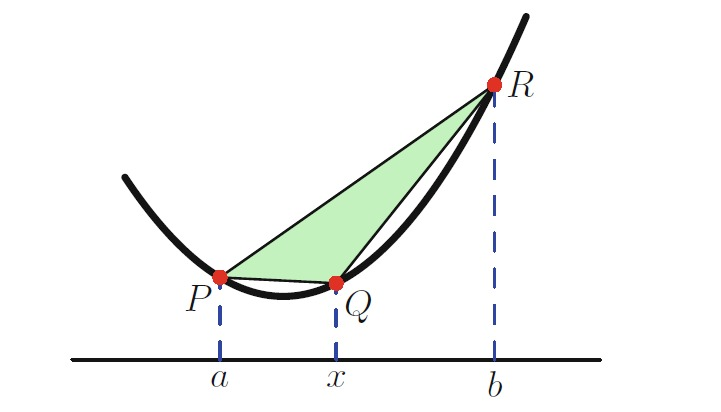
\includegraphics[width=0.5\textwidth]{fig1.3.png}
	\caption{Figura 1.3. panta PQ \(\leq\) panta PR \(\leq \)QR}
\end{figure}


\begin{remark}
Inegalitatea celor trei coarde poate fi \^{i}nt\u{a}rit\u{a} dup\u{a} cum urmeaz\u{a}: 

Dac\u{a} \((f : I \rightarrow \mathbb{R}\) este o func\c{t}ie convex\u{a} , \c{s}i \(x,y,a,b\) sunt puncte ale intervalului I astfel \^{i}nc\^{a}t \(x \leq a, y\leq b, x \neq y\) \c{s}i \(a \neq b\), atunci,
\end{remark}
\begin{displaymath}
   \frac{f\left ( x \right )- f\left ( y \right )}{x-y}\leq \frac{f\left ( a \right )- f\left ( b \right )}{a-b}.
\end{displaymath}
\begin{theorem}
Fie \(f : I \rightarrow \mathbb{R}\) o func\c{t}ie convex\u{a}. Atunci \(f\) are are derivate finite la st\^{a}nga \c{s}i la dreapta \^{i}n orice punct interior al lui I \c{s}i pentru orice \(x <y\) \^{i}n intervalul I avem
\begin{displaymath}
   {f}'_{-}\left ( x \right )\leq {f}'_{+}\left ( x \right )\leq \frac{f\left ( y \right )-f\left ( x \right )}{y-x}\leq {f}'_{-}\left ( y \right )\leq {f}'_{+}\left ( x \right ).
\end{displaymath}
Mai mult, pe intervalul \(I, {f}'_{-}\) este continu\u{a} la st\^{a}nga \c{s}i \({f}'_{+}\) este continu\u{a} la dreapta.
  Prin urmare, dac\u{a} o func\c{t}ie convex\u{a} este diferen\c{t}iabil\u{a} pe intervalul I, atunci aceasta are, de asemenea, derivata continu\u{a}.
\end{theorem}
\begin{proof}
\^{I}ntr-adev\u{a}r, conform inegalit\u{a}\c{t}ii celor trei coarde, avem
\begin{displaymath}
   \frac{f\left ( x \right ) - f\left ( a \right )}{x-a} \leq \frac{f\left ( y \right ) - f\left ( a \right )}{y-a}\leq \frac{f\left ( z \right ) - f\left ( a \right )}{z -a }
\end{displaymath}
pentru orice \(x\leq y\leq a\leq z,\) din I. Acest lucru ne asigur\u{a} faptul c\u{a} exist\u{a} derivat\u{a} la st\^{a}nga \^{i}n a \c{s}i
\begin{displaymath}
   {f}'_{-}\left ( a \right )\geq \frac{f\left ( z \right ) - f\left ( a \right )}{z-a}.
\end{displaymath}

Un argument similar va implica existan\c{t}a lui \({f}'_{+}\left ( a \right )\) \c{s}i  \({f}'_{-}\left ( a \right ) \leq  {f}'_{+}\left ( a \right )\). Pe de alt\u{a} parte, pentru \(x < u\leq v < y\) din intervalul I, aceea\c{s}i inegalitate a celor trei coarde ne conduce la
\begin{displaymath}
   \frac{f\left ( u \right ) - f\left ( x \right )}{u-x}\leq \frac{f\left ( v \right ) - f\left ( x \right )}{v - x}\leq \frac{f\left ( v \right ) - f\left ( y  \right )}{v - y},
\end{displaymath}
deci lu\^{a}nd \(u\rightarrow x+\) \c{s}i \(v\rightarrow y- \), ob\c{t}inem faptul c\u{a} \({f}'_{+}\left ( x \right )\leq {f}'_{-}\left ( y \right ).\)

Pentru continuitatea derivatelor unilaterale, s\u{a} observ\u{a}m c\u{a} din continuitatea lui f pe intervalul I, deducem c\u{a}
\begin{displaymath}
   \frac{f\left ( y \right ) - f\left ( x \right )}{y-x} = \lim_{z \searrow x}\frac{f\left ( y \right ) - f\left ( z \right )}{y-z} \geq \lim_{z\searrow x}{f}'_{+}\left ( z \right )
\end{displaymath}
pentru orice \(x < z < y\). Trec\^{a}nd la limit\u{a}, cum  \(y\searrow x \), ob\c{t}inem,
\begin{displaymath}
 {f}'_{+}\left ( x \right ) \geq  \lim_{z \searrow x } {f}'_{+}\left ( z \right ).
\end{displaymath}
Cum \({f}'_{+}\) este cresc\u{a}toare, r\u{a}m\^{a}ne valabil\u{a} \c{s}i inegalitatea invers\u{a}. Astfel, \({f}'_{+}\)  este  continu\u{a} la dreapta  pe intervalul I. Continuitatea  lui \({f}'_{-}\) la st\^{a}nga poate fi demonstrat\u{a} \^{i}n mod similar.
\end{proof}
Din Teorema 8, orice func\c{t}ie convex\u{a} continu\u{a} \(f:\left [ a,b \right ]\rightarrow \mathbb{R}\) admite derivate unilaterale la capete, care pot fi infinite:
\begin{displaymath}
   - \infty  \leq  {f}'_{+}\left ( a \right ) \leq \infty
\end{displaymath}
\c{s}i
\begin{displaymath}
- \infty  \leq  {f}'_{-}\left ( b \right ) \leq \infty.
\end{displaymath}
Aceast\u{a} teorem\u{a} ne conduce de asemenea la faptul c\u{a} o func\c{t}ie convex\u{a} continu\u{a} \(f:\left [ a,b \right ]\rightarrow \mathbb{R}\) poate fi extins\u{a} la o func\c{t}ie convex\u{a} pe \(\mathbb{R}\) dac\u{a} \c{s}i numai dac\u{a}   \({f}'_{+}\left ( a \right )\) \c{s}i  \( {f}'_{-}\left ( b \right )\)  exist\u{a} \c{s}i sunt finite.

\textbf{C\^{a}t de ”nediferen\c{t}iabil\u{a}” poate fi o func\c{t}ie convex\u{a} ?}

Teorema 8 implic\u{a} faptul c\u{a} orice func\c{t}ie convex\u{a} \(f:I \rightarrow \mathbb{R}\) este derivabil\u{a} cu excep\c{t}ia, eventual, a unei mul\c{t}imi num\u{a}rabile. De fapt, consider\^{a}nd mul\c{t}imea de nediferen\c{t}iabilitate,
\begin{displaymath}
   I_{nd} = \left \{ x : {f}'_{-}\left ( x \right )< {f}'_{+}\left ( x \right ) \right \},
\end{displaymath}
\c{s}i aleg\^{a}nd pentru orice \(x \in I_{nd}\) un num\u{a}r ra\c{t}ional \(r_{x} \in \left ( {f}'_{-}\left ( x \right ),  {f}'_{+}\left ( x \right )  \right )\) vom avea o func\c{t}ie bijectiv\u{a} \(\varphi : x \rightarrow r_{x}\) din \(I_{nd}\) cu valori \^{i}n \(\mathbb{Q}\). \^{I}n consecin\c{t}\u{a}, \(I_{nd}\) este cel mult numrabil\u{a}. S\u{a} observ\u{a}m faptul c\u{a} acest ra\c{t}ionament depinnde de axioma alegerii. 

Teorema 8 ne ofer\u{a} un argument alternativ pentru proprietatea func\c{t}iilor convexe de a fi local Lipschitz pe intervale deschise. 

\^{I}ntr-adev\u{a}r, dac\u{a} \(f : I \rightarrow \mathbb{R}\) este o func\c{t}ie convex\u{a} \c{s}i \(\left [ a,b \right ]\) este un interval compact din interiorul lui I, atunci
\begin{displaymath}
   {f}'_{+}\left ( a \right ) \leq {f}'_{+}\left ( x \right )\leq \frac{f\left ( y \right )- f\left ( x \right )}{y-x}\leq  {f}'_{-}\left ( y \right )\leq {f}'_{-}\left ( b \right )
\end{displaymath}
pentru orice \(x,y \in \left [ a,b \right ]\), cu \(x< y\). 

Prin urmare, \(f|_{\left | a,b \right |}\) verific\u{a} condi\c{t}ia Lipschitz \(\left | f\left ( x \right )  - f\left ( y \right )\right |\leq L\left | x-y \right |,\) cu \(L=\max \left \{ \left | {f}'_{+} \left ( a \right ),{f}'_{-} \left ( b \right ) \right | \right \}\). O consecin\c{t}\u{a} imediat\u{a} este urm\u{a}torul rezultat :

\begin{theorem}
Dac\u{a} \(\left ( f_{n} \right )_{n}\) este un \c{s}ir convergent punctual de func\c{t}ii convexe definite pe un interval deschis I, atunci limita sa f este de asemenea convex\u{a}. Mai mult, convergen\c{t}a este uniform\u{a} pe orice subinterval compact \c{s}i
\begin{displaymath}
   {f}'_{-}\left ( a \right ) \leq \lim_{n\rightarrow \infty } \inf {\left (f_{n}  \right )}'_{-}\left ( a \right )\leq \lim_{n\rightarrow \infty }\sup {\left (f_{n}  \right )}' + \left ( a \right ) \leq {f}'_{+}\left ( a \right ), ~pentru ~orice~ a~ \in I.
\end{displaymath}
\end{theorem}
\begin{proof}
Convexitatea lui f este trivial\u{a}. Din inegalitatea celor trei coarde 1.12, pentru orice \(h >  0\) cu \(a + h \in I\),
\begin{displaymath}
   {\left (f_{n}  \right )}'_{+}\left ( a \right ) \leq  \frac{f_{n}\left ( a + h \right ) - f_{n}\left ( a \right )}{h}
\end{displaymath}
ca urmare
\begin{displaymath}
   \lim_{n\rightarrow \infty } \sup {\left ( f_{n} \right )}'_{+}\left ( a \right ) \leq \lim_{n\rightarrow \infty } \sup \frac{f_{n}\left ( a + h \right ) - f_{n}\left ( a \right )}{h} = \frac{f\left ( a + h \right ) - f\left ( a \right )}{h}.
\end{displaymath}
Lu\^{a}nd \(h\rightarrow 0\), ob\c{t}inem inegalitatea din partea dreapt\u{a} a teoremei 9. Inegalitatea din partea st\^{a}ng\u{a} poate fi demonstrat\u{a} \^{i}n mod similar. 

\c{T}in\^{a}nd cont de o observa\c{t}ie de mai sus despre lipschitzianitatea local\u{a} a  func\c{t}iilor convexe, se poate deduce cu u\c{s}urin\c{t}\u{a} convergen\c{t}a uniform\u{a} pe subintervale compacte ale lui I.
\end{proof}
Este posibil, ca \^{i}n egalitatea de mai sus, egalitatea s\u{a} nu aib\u{a} loc. Pentru a verifica asta, lu\u{a}m \c{s}irul de func\c{t}ii convexe \(f_{n}\left ( x \right ) = \left | x \right |^{1 + \frac{1}{n}}\) care converge pe \(\mathbb{R}\) c\u{a}tre func\c{t}ia \(f\left ( x  \right ) = \left | x \right |.\) 

Evident, \({\left ( f_{n} \right )}'_{+}\left ( 0 \right ) = 0\) pentru orice \(n\) , \^{i}n timp ce \({f}'_{+}\left ( 0 \right ) = 1.\)

Urm\u{a}torul rezultat ne ofer\u{a} o estimare superioar\u{a} a inegalit\u{a}\c{t}ii lui Jensen :

\begin{theorem}
Fie \(f : \left [ a,b \right ] \rightarrow \mathbb{R}\) o func\c{t}ie convex\u{a} \c{s}i
\begin{displaymath}
   \left [ m_{1}, M_{1} \right ],......,\left [ m_{n}, M_{n} \right ]
\end{displaymath}
subintervalele compacte ale lui \(\left [ a,b \right ]\). Fie \(\lambda _{1}, ....,\lambda _{n}\) \^{i}n \(\left [ 0,1 \right ]\) cu \(\sum_{k = 1}^{n}\lambda _{k} = 1.\) Atunci func\c{t}ia
\begin{displaymath}
   E \left ( x_{1},....,x_{n} \right ) = \sum_{k = 1}^{n}\lambda _{k}f\left ( x_{k} \right ) - f\left ( \sum_{k=1}^{n}\lambda _{k}x_{k} \right ),
\end{displaymath}
\^{i}\c{s}i atinge maximul pe \(\Omega = \left [ m_{1}, M_{1} \right ] \times \cdots \times \left [ m_{n}, M_{n} \right ] \)\^{i}ntr-un v\^{a}rf, adic\u{a} \^{i}ntr-un punct \(\{ m_{1}, M_{1} \} \times \cdots \times   \{ m_{n}, M_{n} \}.\)
\end{theorem}
Demonstra\c{t}ia utilizeaz\u{a} urm\u{a}toarea rafinare al teoremei mediilor, a lui Langrange:

\begin{lemma}
Fie \(h : \left [ a,b\right ]\rightarrow \mathbb{R}\) o func\c{t}ie continu\u{a}. Atunci exist\u{a} un punct \(c \in \left ( a,b \right )\) astfel \^{i}nc\^{a}t
\begin{displaymath}
   \underline{D}h\left ( c \right ) \leq  \frac{h\left ( b \right ) - h\left ( a \right )}{b-a}\leq \overline{D}h\left ( c \right ),
\end{displaymath}
unde
\begin{displaymath}
   \underline{\mathcal{D}}h\left ( c \right ) = \lim_{x\rightarrow c}  \frac{h\left ( x \right ) - h\left ( c \right )}{x-c} ~\c{s}i ~ \overline{\mathcal{D}}h\left ( c \right ) = \lim_{x\rightarrow c}  \frac{h\left ( x \right ) - h\left ( c \right )}{x-c},
\end{displaymath}
sunt, derivata inferioar\u{a} respectiv derivata superioar\u{a} a lui h \^{i}n c. 

Conform Teoremei 8, \^{i}n cazul func\c{t}iilor convexe , \(\overline{\mathcal{D}}h\left ( c \right ) = {h}'_{-}\left ( c \right )\)  \c{s}i   \(\overline{\mathcal{D}}h\left ( c \right )  = {h}'_{+}\left ( c \right ).\)
\end{lemma}
\begin{proof}
\^{I}n mod clar, putem presupune faptul c\u{a} f este de asemenea continu\u{a}. Vom demonstra (prin reducere la absurd ) c\u{a}
\begin{displaymath}
  E \left ( x_{1},\cdots, x_{k},\cdots, x_{n} \right ) \leq  \sup \left \{ E\left ( x_{1},\cdots, m_{k},\cdots, x_{n} \right ),\cdots, E\left ( x_{1},....,M_{k},\cdots, x_{n} \right ) \right \},
\end{displaymath}
 pentru orice
\begin{displaymath}
     \left ( x_{1}, x_{2},\cdots, x_{n} \right ) \in\Omega,
\end{displaymath}
\c{s}i orice
\begin{displaymath}
    k \in\left \{ 1,\cdots, n \right \}.
\end{displaymath}
 \^{I}ntr-adev\u{a}r, dac\u{a}
\begin{displaymath}
   E  \left ( x_{1}, x_{2},\cdots, x_{n} \right )  >  \sup \left \{ E\left ( m_{1}, x_{2} ,..., x_{n}\right ),\cdots, E\left ( M_{1}, x_{2} ,..., x_{n}\right )  \right \}
\end{displaymath}
pentru
\begin{displaymath}
  \left ( x_{1}, x_{2},\cdots, x_{n} \right ) \in \Omega,
\end{displaymath}
consider\u{a}m func\c{t}ia
\begin{displaymath}
  h : \left [ m_{1}, M_{1} \right ] \rightarrow \mathbb{R}, h\left ( x \right ) = E\left ( x_{1}, x_{2},...,x_{n} \right ).
\end{displaymath}
Conform lemei 3, exist\u{a} \(\xi \in \left ( m_{1}, x_{1} \right )\) astfel \^{i}nc\^{a}t \(h \left ( x_{1} \right ) - h\left ( m_{1} \right ) \leq  \left ( x_{1} - m_{1} \right )\overline{D}h\left ( \xi  \right ).\)
Cum \(h \left ( x_{1} \right ) >  h\left ( m_{1} \right ),\) rezult\u{a} c\u{a} \(\overline{D}h\left ( \xi  \right ) > 0\), ceea ce este echivalent cu
\begin{displaymath}
   \overline{D}f\left ( \xi  \right ) > \overline{D}f\left (\lambda _{1}\xi +\lambda _{2}\xi +\cdots +\lambda _{n} x_{n} \right ).
\end{displaymath}

Ca urmare, \(\overline{D}f = {f}'_{+}\) este o func\c{t}ie crec\u{a}toare pe \(\left ( a,b \right )\), ceea ce ne conduce la
\begin{displaymath}
   \xi > \lambda _{1}\xi +\lambda _{2}x_{2} + \cdots +\lambda _{n}x_{n},
\end{displaymath}
\c{s}i astfel
\begin{displaymath}
    \xi = \frac{\lambda _{2}x_{2} + \cdots +\lambda _{n}x_{n}}{\lambda _{2}+\cdots +\lambda _{n}}.
\end{displaymath}
Folosind iar lema 3 (aplicat\u{a} de data aceasta lui \(h|_{\left [ x_{1},M_{1} \right ]})\) ob\c{t}inem  existen\c{t}a unui \(\eta \in \left ( x_{1} , M_{1}\right )\) astfel \^{i}nc\^{a}t \(\eta < \frac{\left ( \lambda _{2}x_{2}+\cdots +\lambda _{n}x_{n} \right )}{\lambda _{2}+\cdots +\lambda _{n}}\). Dar asta, contrazice faptul c\u{a} \(\xi <  \eta \).
\end{proof}
\begin{corollary}
Fie \(f : \left [ a,b \right ] \rightarrow \mathbb{R}\) o func\c{t}ie convex\u{a}. Atunci
\begin{displaymath}
   \left ( 1-\lambda  \right )f\left ( a \right ) + \lambda f\left ( b \right ) - f\left ( \left ( 1-\lambda  \right )a + \lambda b \right )\geq \left ( 1-\lambda  \right )f\left ( c \right )+\lambda f\left ( d \right ) - f\left ( \left ( 1 -\lambda \right )c + \lambda d \right ),
\end{displaymath}
pentru orice \(a\leq c\leq d\leq b \)~~\c{s}i \(\lambda \in \left [ 0,1 \right ].\)
\end{corollary}
Fie derivatele, superioar\u{a} \c{s}i inferioar\u{a}, simetrice de ordinul doi ale lui f \^{i}n x, definite de formulele
\begin{displaymath}
   \overline{ \mathcal{D}}^{2}f\left ( x \right ) = \lim_{h\downarrow0} \sup\frac{f\left ( x+h \right ) + f\left ( x-h \right ) -2f\left ( x \right )}{h^{2}}
\end{displaymath}
\begin{displaymath}
   \overline{ \mathcal{D}}^{2}f\left ( x \right ) = \lim_{h\downarrow0} \inf\frac{f\left ( x+h \right ) + f\left ( x-h \right ) -2f\left ( x \right )}{h^{2}}.
\end{displaymath}

Nu este greu s\u{a} verific\u{a}m faptul c\u{a} , dac\u{a} f este derivabil\u{a} de doua ori \^{i}ntr-un punct x, atunci
\begin{displaymath}
   \overline{ \mathcal{D}}^{2}f\left ( x \right ) = \underline{\mathcal{D}}^{2}f\left ( x \right ) = {f}''\left ( x \right ). \label{eq:1.13} \tag{1.13}
\end{displaymath}
\begin{theorem}
Presupunem c\u{a} I este un interval deschis. O func\c{t}ie f cu valoari reale este convex\u{a} pe I dac\u{a} \c{s}i numai dac\u{a} f este continu\u{a} \c{s}i  \(\overline{ \mathcal{D}}^{2}f\geq 0.\)

  Ca o consecin\c{t}\u{a}, dac\u{a} o func\c{t}ie \(f : I \rightarrow \mathbb{R}\) este  func\c{t}ie convex\u{a}  \^{i}ntr-o vecin\u{a}tate a fiec\u{a}rui punct din I, atunci este convex\u{a} pe tot intervalul I.
\end{theorem}
\begin{proof}
Dac\u{a} f este convex\u{a}, atunci, \^{i}n mod clar \(\overline{ \mathcal{D}}^{2}f\geq \underline{\mathcal{D}}^{2}f\geq 0.\) Continuitatea lui f rezult\u{a} din Teorema 1.

Acum, presupunem c\u{a} \(\overline{ \mathcal{D}}^{2}f > 0\) pe I. Dac\u{a} f nu este convex\u{a}, atunci, putem g\u{a}si un punct \(x_{0}\), astfel \^{i}nc\^{a}t \(\overline{ \mathcal{D}}^{2}f \left ( x_{0} \right )\leq 0\), ceea ce ar fi o contradic\c{t}ie. 

De fapt, \^{i}n acest caz, exist\u{a} un subinterval \(I_{0} = \left [ a_{0}, b_{0} \right ]\) astfel \^{i}nc\^{a}t \(f\left ( \frac{a_{0} + b_{0}}{2} \right )> \frac{f\left ( a_{0} \right ) + f\left ( b_{0} \right )}{2}.\) Dac\u{a} ne uit\u{a}m cu aten\c{t}ie, observ\u{a}m faptul c\u{a} unul dintre intervale \(\left [ a_{0}, \frac{a_{0}+b_{0}}{2} \right ], \left [ \frac{\left ( 3a_{0}+b_{0} \right )}{4},\frac{\left ( a_{0}+3b_{0} \right )}{4} \right ],\left [\frac{a_{0}+b_{0}}{2}, b_{0} \right ]\) pot fi alese pentru a \^{i}nlocui intervalul \(I_{0}\) cu un interval mai mic \(I_{1}= \left [ a_{1}, b_{1} \right ], cu  b_{1} -  a_{1}= \frac{b_{0}+ a_{0}}{2}\) \c{s}i \(f\left ( \frac{a_{1}+b_{1}}{2} \right ) > \frac{f\left ( a_{1} \right ) + f\left ( b_{1} \right )}{2}.\) 

Cu ajutorul induc\c{t}iei, vom  putea aplica principiul intervalelor incluse \c{s}i ob\c{t}inem punctul \(x_{0}.\)

\^{I}n cazul general, consider\u{a}m \c{s}irul de func\c{t}ii
\begin{displaymath}
   f_{n}\left ( x \right ) = f\left ( x \right ) + \frac{1}{n}x^{2}.
\end{displaymath}

Avem, \(\overline{ \mathcal{D}}^{2}f _{n} > 0,\) \c{s}i ra\c{t}ionamentul de mai sus ne arat\u{a} c\u{a} \(f _{n}\) este convex\u{a}. 

Evident, \(f _{n}\left ( x \right ) \rightarrow f\left ( x \right )\) pentru orice \(x \in I,\) deci convexitatea lui f este o consecin\c{t}\u{a} a Teoremei 9 de mai sus.
\end{proof}
 \begin{corollary} \textbf{(Testul derivatei a doua)}
  Presupunem c\u{a} \(f : I \rightarrow \mathbb{R}\) este o func\c{t}ie derivabil\u{a} de dou\u{a} ori. Atunci :
\begin{enumerate}
    \item f este convex\u{a} dac\u{a} \c{s}i numai dac\u{a} \({f}''\geq 0\);
    \item  f este strict convex\u{a} dac\u{a} \c{s}i numai dac\u{a} \({f}''\geq 0\) \c{s}i mul\c{t}imea punctelor \^{i}n care \({f}''\) se anuleaz\u{a} nu include intervalele de lungime pozitiv\u{a}.
\end{enumerate}
 \end{corollary}





%
%
%CAPITOLUL 2
%
%


\chapter{Aplica\c{t}ii}

\nocite{steele}
\nocite{pop}
\nocite{siretchi}

Multe dintre func\c{t}iile uzuale ale trigonometriei \c{s}i geometriei au propriet\u{a}\c{t}i de convexitate u\c{s}or de stabilit \c{s}i, de cele mai multe ori, aceas\u{a} convexitate are consecinţe utile.

\begin{problem}(Asupra produsului maxim a dou\u{a} laturi \^{i}ntr-un triunghi)

\^{I}ntr-un triunghi echilateral cu aria A, produsul dintre oricare dou\u{a} laturi este egal cu \(\left (\frac{4}{\sqrt{3}}  \right )\)A. Ar\u{a}ta\c{t}i c\u{a} acesta reprezint\u{a} cazul extrem, mai exact, \^{i}n orice triunghi cu aria A  exist\u{a} dou\u{a} laturi pentru care produsul lungimilor lor este mai mare sau egal cu \(\left (\frac{4}{\sqrt{3}}  \right )A\).
\end{problem}
\begin{proof}
  Pentru a rezolva aceast\u{a} problem\u{a} avem nevoie de formule care s\u{a} lege lungimile laturilor de arie. Cu nota\c{t}iile din figura 1, avem trei astfel de formule:

\begin{displaymath}
  A = \frac{1}{2}ab \sin\gamma = \frac{1}{2}ac \sin \beta = \frac{1}{2}bc \sin \alpha.
\end{displaymath}

\begin{figure}[htbp]
	\centering
	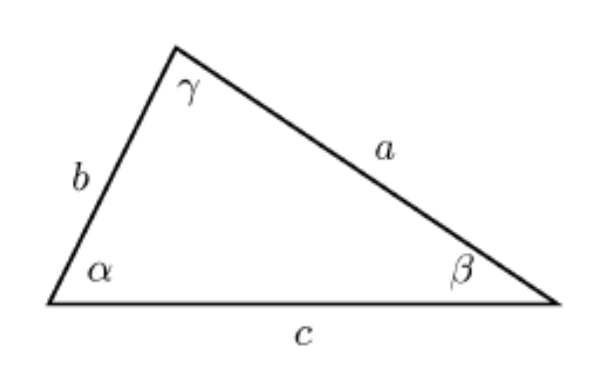
\includegraphics[width=0.5\textwidth]{fig2.1.png}
	\caption{}
\end{figure}

Fig. 1  Toate func\c{t}iile trigonometrice sunt convexe (sau concave) dac\u{a}
argumentele lor sunt limitate la un domeniu adecvat \c{s}i, \^{i}n consecin\c{t}\u{a},
exist\u{a} multe consecin\c{t}e geometrice interesante ale inegalit\u{a}\c{t}ii lui Jensen.


Acum, dac\u{a} facem media acestor reprezent\u{a}ri ale ariei, vom ob\c{t}ine c\u{a}:
\begin{displaymath}
  \frac{1}{3}\left ( ab + ac + bc \right )= \left ( 2A \right )\frac{1}{3}\left \{ \frac{1}{sin \alpha } + \frac{1}{sin \beta } + \frac{1}{sin \gamma }\right \}, \label{eq:2.1} \tag{2.1}
\end{displaymath}
\c{s}i aceasta este o formul\u{a} care ne conduce la a studia convexitatea func\c{t}iei \(\frac{1}{sin x}\). Reprezentarea grafic\u{a} a acesteia, \(x \mapsto \frac{1}{sin x}\), pentru \(x\in \left ( 0, \infty  \right )\) cu siguran\c{t}\u{a} este convex\u{a}, iar presupunerea noastr\u{a} poate fi confirmat\u{a} prin calcularea derivatei a doua,
\begin{displaymath}
  {\left ( \frac{1}{sin x} \right )}''= \frac{1}{sin x} + 2\frac{cos^{2}x}{sin ^{3}x}> 0~~ \text{pentru orice}~~ x\in \left ( 0, \pi  \right )  \label{eq:2.2} \tag{2.2}
\end{displaymath}

  Prin urmare, din moment ce avem \[\frac{\left ( \alpha + \beta  + \gamma  \right )}{3}= \frac{\pi }{3},\] rezult\u{a} din inegalitatea lui Jensen c\u{a}
\begin{displaymath}
  \frac{1}{3}\left \{ \frac{1}{sin \alpha }  + \frac{1}{sin \beta } + \frac{1}{sin \gamma }\right \}\geq \frac{1}{sin \frac{\pi }{3}} =  \frac{2}{\sqrt{3}},
\end{displaymath}
deci, folosind inegalitatea \ref{eq:2.1}, ob\c{t}inem estimarea cerut\u{a}
\begin{displaymath}
 \max \left ( ab, ac, bc \right )\geq \frac{1}{3}\left ( ab + ac + bc \right )\geq \frac{4}{\sqrt{3}}A. \label{eq:2.3} \tag{2.3}
\end{displaymath}

\end{proof}
\begin{remark}
Aceast\u{a} problem\u{a} este str\^{a}ns legat\u{a} de o inegalitate binecunoscut\u{a} a lui Weitzenböck care afirm\u{a} c\u{a} \^{i}n orice triunghi avem
\begin{displaymath}
  a^{2} + b^{2} + c^{2} \geq \frac{4}{\sqrt{3}}A. \label{eq:2.4} \tag{2.4}
\end{displaymath}

De fapt, pentru a trece de la inegalitatea \ref{eq:2.3} la inegalitatea lui Weitzenböck trebuie doar s\u{a} ne amintim c\u{a}
\begin{displaymath}
  ab + ac + bc \leq a^{2} + b^{2} + c^{2},
\end{displaymath}
care este o inegalitate bine cunoscut\u{a} pe care o putem ob\c{t}ine \^{i}n dou\u{a} moduri  - folosind inegalitatea lui Cauchy sau folosind inegalitatea MA-MG

  Inegalitatea lui Weitzenböck se dovede\c{s}te a avea multe demonstra\c{t}ii instructive - Engel (1998) a dat unsprezece!
Exist\u{a} c\^{a}teva metode matematice pe care le-am putea numi generic "improvers"; \^{i}n linii mari, acestea sunt metode care pot fi utilizate \^{i}ntr-un mod algoritmic pentru a generaliza o identitate, sau pentru a \^{i}mbun\u{a}t\u{a}\c{t}i un rezultat dat.
\end{remark}
Urm\u{a}toarea problem\u{a} ofer\u{a} un exemplu de alt fel. Aceasta sugereaz\u{a} cum am putea \^{i}mbun\u{a}t\u{a}\c{t}i aproape orice rezultat care a fost ob\c{t}inut folosind inegalitatea lui Jensen.

\begin{problem}
(Formula defectului a lui Hölder)

Dac\u{a} \(f : \left [ a,b  \right ] \to \mathbb{R}\) este derivabil\u{a} de doua ori \c{s}i
\begin{displaymath}
  0 \leq m \leq  f''\left ( x \right ) \leq  M,~ \text{pentru orice }~x\in \left [ a,b \right ], \label{eq:2.5} \tag{2.5}
\end{displaymath}
atunci pentru orice  \(a\leq x_{1}\leq x_{2}\leq ....\leq x_{n} \leq b \) \c{s}i orice numere reale pozitive \(p_{k}, k= 1,2,.....,n \) cu \(p_{1} + p_{2} + \cdots+ p_{n} = 1\),  exist\u{a}  \(\mu \in \left [ m, M \right ]\) pentru care are loc egalitatea
\begin{displaymath}
  \sum_{k = 1}^{n}p_{k}f\left ( x_{k} \right ) - f\left ( \sum_{k = 1}^{n} p_{k}x_{k}\right ) = \frac{1}{4}\mu \sum_{j = 1}^{n}\sum_{k = 1}^{n}p_{j}p_{k}\left ( x_{j} - x_{k} \right )^{2}. \label{eq:2.6} \tag{2.6}
\end{displaymath}
\end{problem}
\begin{remark}
Acest rezultat provine din aceea\c{s}i lucrare faimoas\u{a} din 1885 a lui Otto Ludwig Hölder (1859 - 1937) \^{i}n care se g\u{a}seşte demonstra\c{t}ia inegalit\u{a}ţii care are a ajuns s\u{a} fie cunoscut\u{a}  ca ”inegalitatea lui Hölder”. Formula defectului \ref{eq:2.6} este mult mai pu\c{t}in cunoscut\u{a}, dar este totu\c{s}i valoroas\u{a}. Aceasta ofer\u{a} o m\u{a}sur\u{a} perfect natural\u{a} a diferen\c{t}ei dintre cele dou\u{a} p\u{a}r\c{t}i ale inegalit\u{a}\c{t}ii lui Jensen \c{s}i ne spune cum s\u{a} \^{i}nvingem versiunea  inegalit\u{a}\c{t}ii lui Jensen ori de c\^{a}te ori putem verifica ipoteza suplimentar\u{a} \ref{eq:2.5}.
\^{I}n mod similar, dac\u{a} M este mic, s\u{a} spunem \(0 \leq M \leq \epsilon\), atunci inegalitatea \ref{eq:2.5} ne spune c\u{a} f se comport\u{a} mai degrab\u{a} ca o func\c{t}ie afin\u{a}, \(f\left ( x \right ) = \alpha  + \beta x\). Pentru o func\c{t}ie afin\u{a}, partea st\^{a}ng\u{a} a egalitatii \ref{eq:2.6} este identic egal\u{a} cu zero, dar \^{i}n general, rela\c{t}ia \ref{eq:2.6} afirm\u{a} ceva mai subtil. Mai precis, ne spune c\u{a} partea st\^{a}ng\u{a} este un mic multiplu al unei expresii  \^{i}n care valorile \(x_{j}, j = 1,2,\cdots ,n \) sunt r\u{a}spandite pe \^{i}ntreg intervalul \(\left [ a, b \right ]. \)
\end{remark}
\begin{proof}
Aceast\u{a} problem\u{a} ne duce \^{i}n mod firesc la urm\u{a}toarea \^{i}ntrebare: Cum putem folosi faptul c\u{a} \(0\leq m\leq {f}''\left ( x \right )\leq M \)?

Odata ce ne-am pus aceast\u{a} \^{i}ntrebare, s-ar putea s\u{a} nu fie nevoie de mult pentru a observa c\u{a} cele dou\u{a} func\c{t}ii
\begin{displaymath}
  g\left ( x \right ) = \frac{1}{2}Mx^{2} - f\left ( x \right )~~ \c{s}i~~
h\left ( x \right ) = f\left ( x \right ) - \frac{1}{2}mx^{2}
\end{displaymath}
sunt dou\u{a} func\c{t}ii convexe.
Aceast\u{a} observa\c{t}ie ne \^{i}ndeamn\u{a} s\u{a} ne \^{i}ntreb\u{a}m ce spune inegalitatea lui Jensen despre aceste func\c{t}ii.\\
Pentru \(g\left ( x \right )\), inegalitatea lui Jensen ne d\u{a} m\u{a}rginirea
\begin{displaymath}
  \frac{1}{2}M\bar{x}^{2} - f\left ( \bar{x} \right )\leq \sum_{k = 1}^{n}p_{k}\left \{ \frac{1}{2}Mx_{k}^{2} - f\left ( x_{k} \right )\right \}
\end{displaymath}
unde am notat \(\bar{x} = p_{1}x_{1}+ p_{2}x_{2}+ \cdots + p_{n}x_{n}\) \c{s}i aceast\u{a} inegalitate este u\c{s}or de rearanjat  pentru a ob\c{t}ine
\begin{displaymath}
  \left \{ \sum_{k = 1}^{n} p_{k}f\left ( x_{k} \right )\right \} - f\left (\bar{x}  \right )\leq \frac{1}{2}M\left \{ \left ( \sum_{k=1}^{n} p_{k}x_{k}^{2}\right ) - \bar{x}^{2} \right \} = \frac{1}{2}M\sum_{k = 1}^{n}p_{k}\left ( x_{k} - \bar{x} \right )^{2}.
\end{displaymath}

Un calcul analog pentru  \(h\left ( x \right )\) ne ofer\u{a} o limit\u{a} inferioar\u{a}
\begin{displaymath}
  \left \{ \sum_{k = 1}^{n} p_{k}f\left ( x_{k} \right )\right \} - f\left (\bar{x}  \right )\geq \frac{1}{2}m\sum_{k = 1}^{n}p_{k}\left ( x_{k} - \bar{x} \right )^{2}
\end{displaymath}
\c{s}i aceste limite, cea superioar\u{a} \c{s}i cea inferioar\u{a} aproape completeaz\u{a} demonstra\c{t}ia egalit\u{a}\c{t}ii  \ref{eq:2.6}. Singurul lucru care lipse\c{s}te este identitatea
\begin{displaymath}
  \sum_{k = 1}^{n}p_{k}\left ( x_{k} - \bar{x} \right )^{2} = \frac{1}{2}\sum_{j = 1}^{n}\sum_{k = 1}^{n} p _{j}p_{k}\left ( x_{j} - x_{k} \right )^{2}
\end{displaymath}
care se poate verifica usor prin calcul direct folosind defini\c{t}ia lui \(\bar{x}\).
\end{proof}
Convexitatea \c{s}i inegalitatea lui Jensen ofer\u{a} solu\c{t}ii simple pentru multe probleme.
  Urm\u{a}toarea problem\u{a} vine din celebra sec\c{t}iune cu probleme a ”American Mathematical Monthly” \c{s}i ofer\u{a} un exemplu clasic al acestei afirma\c{t}ii.
  La \^{i}nceput problema pare destul de u\c{s}oar\u{a}, dar, cur\^{a}nd, \^{i}ntampin\u{a}m dificult\u{a}\c{t}i.

\begin{problem}(AMM 2002, Proposed by M. Mazur)\\
Ar\u{a}ta\c{t}i c\u{a} dac\u{a} a,b \c{s}i c, sunt numere reale pozitive care verific\u{a} \(abc \geq 2^{9}\), atunci
\begin{displaymath}
  \frac{1}{\sqrt{1 + \left ( abc \right )^{\frac{1}{3}}}}\leq \frac{1}{3}\left \{ \frac{1}{\sqrt{1 + a}} + \frac{1}{\sqrt{1 + b}} + \frac{1}{\sqrt{1 + c}}\right \}     
  \label{eq:2.7} \tag{2.7}
\end{displaymath}
\end{problem}
\begin{proof}
Media din partea dreapt\u{a} sugereaz\u{a} faptul c\u{a} inegalitatea lui Jensen s-ar putea dovedi util\u{a}, \^{i}n timp ce media geometric\u{a} din partea st\^{a}ng\u{a} sugereaz\u{a} c\u{a} func\c{t}ia exponen\c{t}ial\u{a} va avea un rol.

Dac\u{a} ne uit\u{a}m mai atent, putem observa c\u{a}
\begin{displaymath}
  f\left ( x \right ) = \frac{1}{\sqrt{1+ e^{x}}}
\end{displaymath}
ne poate ajuta la folosirea inegalit\u{a}\c{t}ii lui Jensen. De fapt, odat\u{a} ce am scris aceast\u{a} func\c{t}ie, se poate verifica aproape f\u{a}r\u{a} calcul c\u{a} inegalitatea propus\u{a} \ref{eq:2.7} este echivalent\u{a} cu
\begin{displaymath}
  f\left ( \frac{x + y + z}{3} \right )\leq \frac{1}{3}\left \{ f\left ( x \right ) + f\left ( y \right ) + f\left ( z \right ) \right \}    \label{eq:2.8} \tag{2.8}
\end{displaymath}
pentru orice $x, y, z$ astfel \^{i}nc\^{a}t \(\exp\left ( x + y + z \right )\geq 2^{9}.\)

Pentru a vedea dac\u{a} putem aplica inegalitatea lui Jensen, trebuie s\u{a} evalu\u{a}m convexitatea lui f. \^{I}ntr-adevar, avem

\begin{figure}[htbp]
	\centering
	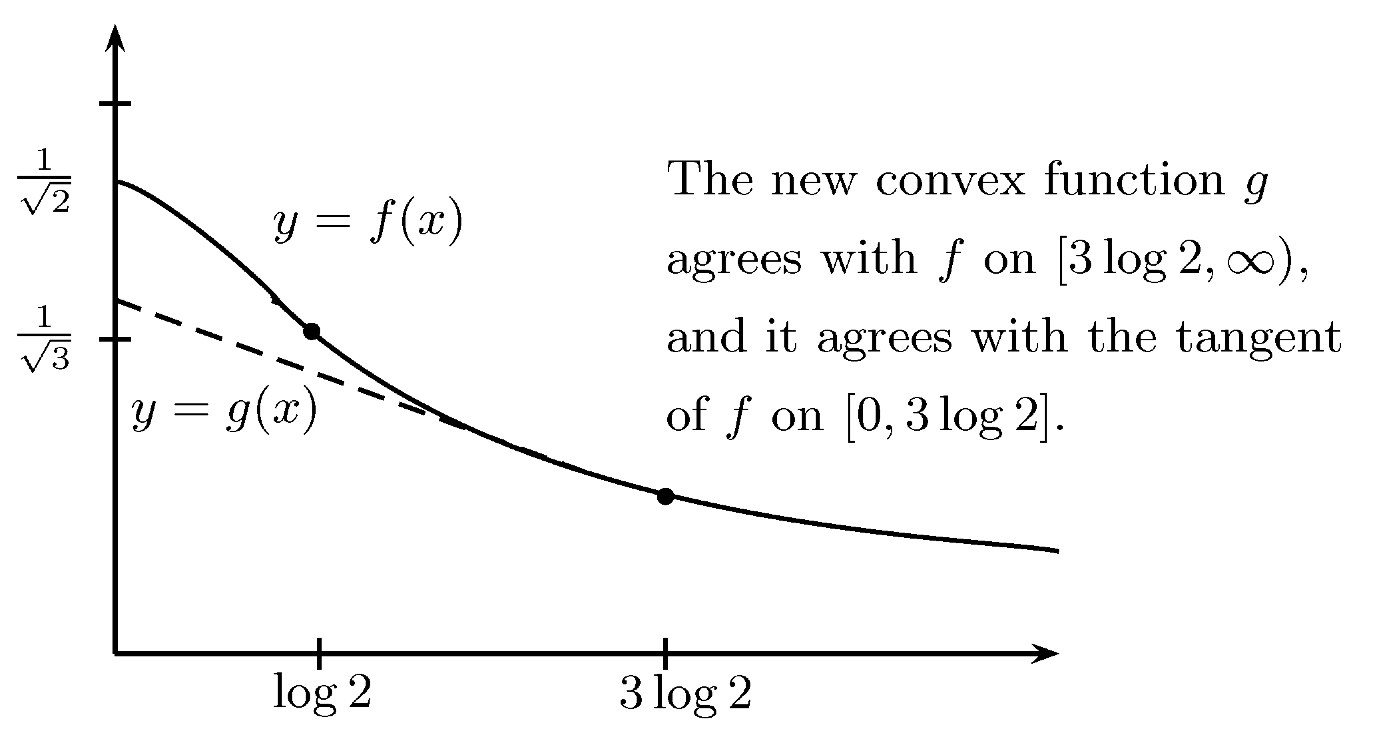
\includegraphics[width=0.5\textwidth]{fig_pb3.png}
	\caption{Figura 1.3. Utilizarea eficient\u{a} a inegalit\u{a}\c{t}ii lui Jensen necesit\u{a} g\u{a}sirea unei func\c{t}ii care este convex\u{a} pe \(\left [ 0, \infty  \right )\)  \c{s}i care nu este niciodat\u{a} mai mare dec\^{a}t f.}
\end{figure}

\begin{displaymath}
  {f}'\left ( x \right ) = -\frac{e^{x}}{2 \left ( 1 + e^{x} \right )^{\frac{3}{2}}}
\end{displaymath}
si
\begin{displaymath}
  {f}''\left ( x \right ) = -\frac{1}{2}\left (  1 + e^{x} \right )^{-\frac{3}{2}}e^{x} + \frac{3}{4}\left ( 1 + e^{x} \right )^{-\frac{5}{2}}e^{2x}
\end{displaymath}

Cea de a doua egalitate ne arat\u{a} c\u{a} \({f}''\left ( x \right ) \geq 0\) dac\u{a} \c{s}i numai dac\u{a} avem \(e^{x}\geq 2\), astfel \^{i}nc\^{a}t cu ajutorul inegalit\u{a}\c{t}ii lui Jensen  constat\u{a}m c\u{a} inegalitatea ini\c{t}iala \ref{eq:2.7}  este adevarat\u{a} cu condi\c{t}ia ca fiecare dintre termenii a, b \c{s}i c s\u{a} fie mai mari sau egali cu 2.

Dificultatea cu care ne confrunt\u{a}m aici este c\u{a} ipoteza problemei  ne spune doar  c\u{a} produsul \(abc\) este mai mare sau egal cu \(2^{9}\); nu ni se da nicio  limit\u{a} pentru termenii  individuali, cu excep\c{t}ia faptului c\u{a} \( a > 0, b > 0 \) \c{s}i \(c > 0\) . Astfel, inegalitatea lui Jensen nu poate completa demonstra\c{t}ia de la sine \c{s}i noi trebuie s\u{a} caut\u{a}m alte informa\c{t}ii.

Exist\u{a} multe idei pe care le-am putea \^{i}ncerca, dar inainte de a merge prea departe,  ar trebui s\u{a} lu\u{a}m \^{i}n considerare graficul lui \(f\left ( x \right )\). Ceea ce  g\u{a}sim  din graficul  reprezentat \^{i}n figura 3 este c\u{a} \(f\left ( x \right ) \) arat\u{a} convex\u{a} pe interval \(\left [ 0, 10 \right ]  \), \^{i}n ciuda faptului c\u{a} calculul care arat\u{a} c\u{a} \(f\left ( x \right ) \) este concav\u{a} pe \(\left [ 0, \log _{} 2\right ] \) \c{s}i convex\u{a} pe \(\left [ \log _{} 2 , \infty \right ) \). Astfel, graficul nostru ofer\u{a} o noua speran\c{t}\u{a}; poate c\u{a} o mica modificare a lui \(f\) ar putea conduce la convexitatea de care noi avem nevoie pentru a rezolva problema.

C\^{a}nd ne gandim la modul \^{i}n care am sperat s\u{a} folosim \(f\) cu inegalitatea lui Jensen, \^{i}n cur\^{a}nd ne d\u{a}m seama c\u{a} ne putem u\c{s}ura pu\c{t}in sarcina. S\u{a} presupunem, de exemplu, c\u{a} putem gasi o func\c{t}ie convex\u{a} \(g : \left [ 0 , \infty  \right ) \to \mathbb{R}\) astfel \^{i}nc\^{a}t s\u{a} avem  condi\c{t}iile:
\begin{displaymath}
  g\left ( x \right ) \leq  f\left ( x  \right ),~~ \text{pentru orice}~~ x \in  \left [ 0 , \infty  \right )    \label{eq:2.9} \tag{2.9}
\end{displaymath}
\c{s}i condi\c{t}ia complementar\u{a}
\begin{displaymath}
  g \left ( x \right ) = f \left ( x \right ), ~~ \text{pentru orice }~~  x\geq 3 \log 2. \label{eq:2.10} \tag{2.10}
\end{displaymath}

Pentru o astfel de func\c{t}ie, inegalitatea lui Jensen ne spune  c\u{a} dac\u{a} x,y \c{s}i z verific\u{a} \[exp \left ( x + y + z \right )\geq  2^{9} \] avem inegalit\u{a}\c{t}ile
\begin{displaymath}
\begin{split}
  f\left ( \frac{x + y + z}{3} \right ) &= g\left ( \frac{x + y + z}{3} \right )\\
   &\leq  \frac{1}{3}\left \{ g\left ( x \right ) + g\left ( y \right ) + g\left ( z \right ) \right \} \\ & \leq  \frac{1}{3}\left \{ f\left ( x \right ) + f\left ( y \right ) + f\left ( z \right ) \right \}.
  \end{split}
\end{displaymath}

Primul \c{s}i ultimul termen al acestei inegalit\u{a}\c{t}i conduc la inegalitatea \ref{eq:2.8}, deci solu\c{t}ia problemei ar fi complet\u{a}, cu excep\c{t}ia unui mic detaliu — mai trebuie s\u{a} ar\u{a}t\u{a}m c\u{a} exist\u{a} o func\c{t}ie  g convex\u{a} pe \( \left [ 0 , \infty  \right ) \) astfel \^{i}nc\^{a}t  \(g\left ( x \right ) \leq  f\left ( x \right )\) pentru orice  \(x \in \left [ 0 , 3\log 2 \right ]\) \c{s}i \( f\left ( x \right ) = g\left ( x \right )\) pentru orice \( x \geq 3\log 2\).

O modalitate de a construi o func\c{t}ie convex\u{a} \(g\) cu propriet\u{a}\c{t}ile  descrise mai sus este, s\u{a} lu\u{a}m  \(g\left ( x \right ) = f\left ( x \right )\) pentru \(x \geq  3\log2\) \c{s}i s\u{a} definim \(g\left ( x \right )\) pe \(\left [ 0 , 3\log 2 \right ]\) prin extrapolare liniar\u{a}. Astfel, pentru \(x\in \left [ 0 , 3\log 2 \right ]\), lu\u{a}m
\begin{equation} \nonumber
    \begin{split}
     g\left ( x \right )  &      = f\left ( 3\log 2 \right ) + \left ( x - 3\log 2 \right ){f}'\left ( 3\log2 \right ) \\ &  = \frac{1}{3} + \left ( 3\log2 - x  \right )\left ( \frac{4}{27} \right )
    \end{split}
\end{equation}

Trei observa\c{t}ii simple sunt acum suficiente pentru a demonstra c\u{a} \(g\left ( x \right )\leq f\left ( x \right )\), pentru orice \(x\geq 0\). Pentru \^{i}nceput, pentru \(x\geq 3\log 2\), avem \(g\left ( x \right ) = f\left ( x \right )\) din defini\c{t}ie.

Cea de a doua observa\c{t}ie, pentru \(\log 2 \leq  x \leq  3\log 2\) avem  \(g( x )\leq f\left ( x \right ) \) pentru c\u{a} aici  \(g\left ( x \right )\) are valoarea unei drepte tangente la \((f\left ( x \right )\) \c{s}i din convexitatea lui f pe \(\log 2 \leq  3 \leq 3\log 2\) dreapta tangent\u{a} este sub f.

Cea de a treia observa\c{t}ie; \^{i}n regiunea critic\u{a} \(0\leq  x \leq \log2\), avem \(g\left ( x \right ) \leq  f\left ( x \right )\) deoarece,
\begin{enumerate}
  \item f este concav\u{a},
  \item g este liniar\u{a},
  \item f este mai mare dec\^{a}t \(g\) la capetele intervalului \(\left [ 0 , \log 2 \right ]\).
\end{enumerate}
Mai precis, avem
\begin{displaymath}
  g\left ( 0 \right ) = 0.641\cdots \leq f\left ( 0 \right ) = \frac{1}{\sqrt{2}} = 0.707\cdots,
\end{displaymath}
\^{i}n timp ce \^{i}n cel de-al doilea punct avem
\begin{displaymath}
  g\left ( \log 2 \right ) = 0.538\cdots  \leq f\left ( \log2 \right ) = \frac{1}{\sqrt{3}} = 0.577\cdots.
\end{displaymath}
Astfel, func\c{t}ia convex\u{a} \(g\) este \^{i}ntr-adevar un minorant al func\c{t}iei \(f\) care se afl\u{a} \^{i}n concordan\c{t}\u{a} cu \(f\) pe \(\left [ 3\log 2 , \infty  \right )\), a\c{s}adar rezolvarea problemei este complet\u{a}.
\end{proof}
\begin{problem} (O inegalitate renascentist\u{a})\\
   Matematicianul renascentist Pietro Mengoli (1625 – 1686) a avut nevoie doar de algebra elementar\u{a} pentru a demonstra inegalitatea
 \begin{displaymath}
   \frac{1}{x - 1} + \frac{1}{x} + \frac{1}{x + 1} > \frac{3}{x} , ~~ \text{pentru orice } ~~  x > 1, \label{eq:2.11} \tag{2.11}
 \end{displaymath}
totu\c{s}i, a ob\c{t}inut o revendicare asupra nemuririi intelectuale atunci c\^{a}nd a folosit asta pentru a oferi una dintre cele mai timpurii dovezi ale divergen\c{t}ei seriilor armonice,
\begin{displaymath}
  H_{n} = 1 + \frac{1}{2} + \frac{1}{3} + \cdots + \frac{1}{n} \Rightarrow \lim_{n \to \infty } H_{n} = \infty \label{eq:2.12} \tag{2.12}
\end{displaymath}

Redescoperi\c{t}i demonstra\c{t}ia algebric\u{a} a inegalit\u{a}\c{t}ii lu Mengoli 2.11 \c{s}i verifica\c{t}i faptul c\u{a} rezult\u{a} \c{s}i din inegalitatea lui Jensen. Mai departe, ar\u{a}ta\c{t}i, cum a facut Mengoli, faptul c\u{a} inegalitatea \ref{eq:2.11} implic\u{a} divergen\c{t}a lui \(H_{n}\) .
\end{problem}
\begin{proof}
Simplific\^{a}nd \(\frac{1}{x}\) din ambele p\u{a}r\c{t}i \c{s}i adun\^{a}nd frac\c{t}iile se vede c\u{a} inegalitatea lui Mengoli este echivalent\u{a} cu inegalitatea  trivial\u{a} \(x^{2} >  x^{2} – 1\). \\
Pentru o demonstra\c{t}ie folosind inegalitatea lui Jensen, observ\u{a}m c\u{a} \(x \mapsto \frac{1}{x}\) este stict convex\u{a}. Aplic\u{a}m inegalitatea lui Jensen pentru $x_1=x-1,$ $x_2=x,$ $x_3=x-1,$ si $\lambda_i=1/3,~i=1, 2, 3:$
\[
f\biggl(\frac{1}{3}(x-1+x+x+1)\biggr)=f(x)<\frac{1}{3}f(x+1)+\frac{1}{3}f(x)+\frac{1}{3}f(x-1)\Leftrightarrow
\]
\[
\frac{1}{x}<\frac{1}{3}\frac{1}{x+1}+\frac{1}{3}\frac{1}{x}+\frac{1}{3}\frac{1}{x-1}
\]
care inmul\c{t}it\u{a} cu trei este inegalitatea lui Mengoli.\\
\^{I}n final, pentru o versiune modern\u{a} a demonstra\c{t}iei lui Mengoli c\u{a} \(H_{n}\) diverge, presupunem prin absurd c\u{a} \(H_{\infty }< \infty\) \c{s}i scriem \(H_{\infty }\) c\u{a}
\begin{displaymath}
  1 + \left ( \frac{1}{2} + \frac{1}{3} + \frac{1}{4} \right ) + \left ( \frac{1}{5} + \frac{1}{6} + \frac{1}{7} \right ) + \left ( \frac{1}{8} + \frac{1}{9} +\frac{1}{10} \right )+\cdots.
\end{displaymath}

Acum, prin aplicarea inegalit\u{a}\c{t}ii lui Mengoli \^{i}n cadrul grupurilor formate g\u{a}sim c\u{a}
\[
H_{\infty }>1 + \frac{3}{3} + \frac{3}{6} + \frac{3}{9} + ..= 1 + H_{\infty }
\]
care ne conduce la contradic\c{t}ia \(H_{\infty } > 1 + H_{\infty }\).
\end{proof}
\begin{remark}
Potrivit lui Havil, Mengoli a fost cel care a propus pentru prima data problema determin\u{a}rii valorii sumei \[1 + \frac{1}{2^{2}} + \frac{1}{3^{2}} + \cdots.\]
Problema a rezistat eforturilor celor mai buni matematicieni ai Europei p\^{a}n\u{a} \^{i}n anul 1731 c\^{a}nd L. Euler a determinat valoarea ca fiind \(\frac{\pi^{2}}{6}\).
\end{remark}

\begin{problem}
Ar\u{a}ta\c{t}i c\u{a} dac\u{a} \(x , y , z > 0\) si \(x+ y + z = 1\), atunci
\begin{displaymath}
  64 < \left ( 1 + \frac{1}{x} \right )\left ( 1 + \frac{1}{y} \right )\left ( 1 + \frac{1}{z} \right ).
\end{displaymath}
\end{problem}
\begin{proof}
Inegalitatea rezult\u{a} prin aplicarea inegalit\u{a}\c{t}ii lui Jensen func\c{t}iei
\begin{displaymath}
  f\left ( t \right ) = \ln \left ( 1+\frac{1}{t} \right ) = \ln \left ( 1 + t \right ) - \ln \left ( t \right ),~t>0
\end{displaymath}
care este strict convex\u{a} deoarece
\begin{displaymath}
  {f}''\left ( t \right ) = -\frac{1}{\left ( 1 + t \right )^{2}} + \frac{1}{t^{2}} > 0,  \text{pentru orice } t > 0.
\end{displaymath}

\^{I}ntr-adevar, pentru  $x_1=x,$ $x_2=y,$ $x_3=z,$ si $\lambda_i=1/3,~i=1, 2, 3:$
\[
f\biggl(\frac{1}{3}(x+y+z)\biggr)=f\biggl(\frac{1}{3}\biggr)<\frac{1}{3}f(x)+\frac{1}{3}f(y)+\frac{1}{3}f(z)\Leftrightarrow
\]
\[
\ln (4)<\frac{1}{3}\ln\biggl(1+\frac{1}{x})\biggr) +\frac{1}{3}\ln\biggl(1+\frac{1}{y}\biggr)+\frac{1}{3}\ln\biggl(1+\frac{1}{z}\biggr)\Leftrightarrow
\]
\[
3\ln (4)< \ln\biggl((1+\frac{1}{x})(1+\frac{1}{y})(1+\frac{1}{z})\biggr)
\]
\c{s}i aplic\^{a}nd exponen\c{t}iala ob\c{t}inem inegalitatea dorit\u{a}.
\end{proof}


\begin{problem} (Inegalitatea ariei n-poligonului)

Figura 4 sugereaz\u{a} c\u{a}  dintre toate poligoanele convexe cu n laturi care pot fi \^{i}nscrise \^{i}ntr-un cerc, numai n-gonul regulat are aria maxim\u{a}. Poate inegalitatea lui Jensen s\u{a} fie folosit\u{a} pentru a confirma aceast\u{a} afirma\c{t}ie?

\begin{figure}[htbp]
	\centering
	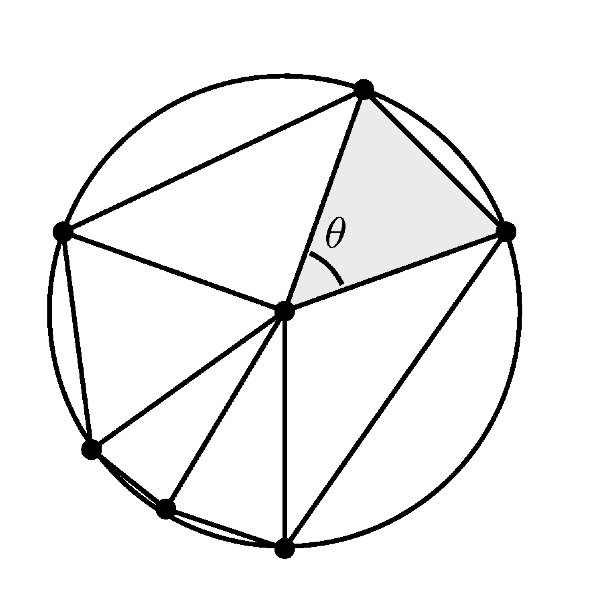
\includegraphics[width=0.5\textwidth]{fig_pb6.png}
	\caption{Figura 4. Dac\u{a} un poligon convex cu n laturi este \^{i}nscris \^{i}n cercul unitar, imagina\c{t}ia noastr\u{a} vizual\u{a} sugereaz\u{a} c\u{a} aria este maximizat\u{a} doar de un poligon regulat. Aceast\u{a} presupunere poate fi dovedit\u{a} prin metode care le-ar fi fost familiare lui Euclid, dar o demonstra\c{t}ie mai modern\u{a} prin convexitate este mai u\c{s}oar\u{a}.}
\end{figure}


\end{problem}
\begin{proof}
Din figura geometric\u{a} precizat\u{a}, dac\u{a} presupunem f\u{a}r\u{a} a restrange generalitatea c\u{a} raza cercului este 1, aria A a unui poligon \^{i}nscris cu n laturi poate fi scris\u{a} ca
\begin{displaymath}
  A = \frac{1}{2}\sum_{k = 1}^{n} \sin \theta _{k} ~~\text{unde} ~~0< \theta _{k} ~~\text{\c{s}i}~~ \sum_{k = 1}^n{\theta _{k}} = 2\pi.
\end{displaymath}
  Cum func\c{t}ia  \(\sin \left ( \cdot  \right )\) este strict concav\u{a} pe \(\left [ 0 , \pi  \right ]\), folosind inegalitatea lui Jensen avem
\begin{displaymath}
  A = \frac{1}{2}\sum_{k = 1}^{n} \sin \theta _{k}  \leq \frac{1}{2}n\sin\left ( \frac{1}{n}\sum_{k = 1}^{n}\theta _{k} \right ) = \frac{1}{2}n\sin \left ( \frac{2\pi }{n} \right ) = {A}'
\end{displaymath}
\c{s}i avem egalitate dac\u{a} \c{s}i numai dac\u{a} \(\theta _{k} = \frac{2\pi }{n}\) pentru orice \(1\leq k\leq n\). Cum \({A}'\) este aria unui n-poligon regulat \^{i}nscris, optimalitatea presupus\u{a} este confirmat\u{a}.
\end{proof}

\begin{problem} (Inegalit\u{a}\c{t}ile investi\c{t}ionale)

Dac\u{a} \(0< r_{k} < \infty\). Dac\u{a} investi\c{t}ia noastr\u{a} de un dolar \^{i}n anul \(k\) cre\c{s}te la \(1 +  r_{k}\) dolari la sf\^{a}r\c{s}itul anului, numim \(r_{k}\) dob\^{a}nda investit\u{a}\c{t}iei \^{i}n anul \(k\). Demonstra\c{t}i c\u{a} valoarea
\begin{displaymath}
  V = \left ( 1 + r_{1} \right )\left ( 1 + r_{2} \right )\cdots \left ( 1 + r_{n} \right )
\end{displaymath}
a investi\c{t}iei noastre dup\u{a} n ani verific\u{a} inegalit\u{a}\c{t}ile
\begin{displaymath}
  \left ( 1 + r_{G} \right )^{n} \leq \prod_{k = 1}^{n} \left ( 1 + r_{k} \right )\leq \left ( 1 + r_{A} \right )^{n}, \label{eq:2.13} \tag{2.13}
\end{displaymath}
unde
\begin{displaymath}
  r_{G} = \left ( r_{1}r_{2} \cdots r_{n}\right )^{\frac{1}{n}}~~ \c{s}i~~ r_{A} = \frac{\left ( r_{1} + r_{2} +  \cdots+ r_{n}\right )}{n}.
\end{displaymath}
De asemenea explica\c{t}i de ce aceaste inegalit\u{a}\c{t}i  pot fi vazute ca un rafinament al inegalit\u{a}\c{t}ii MA-MG.
\end{problem}
\begin{proof}
Evident, inegalitatea din dreapta rezult\u{a} imediat dac\u{a} aplic\u{a}m inegalitatea MA-MG pentru
\begin{displaymath}
  a_{k} = 1 + r_{k},~ k =1,2,\cdots, n.
\end{displaymath}
Pentru inegalitatea din partea st\^{a}ng\u{a} aplic\u{a}m inegalitatea lui Jensen aplicat\u{a} func\c{t}iei convexe
\[x \mapsto \ln\left ( 1 + e^{x} \right ).\]
Evident, dac\u{a} not\u{a}m cu $f$ aceast\u{a} func\c{t}ie, observ\u{a}m c\u{a}
\[
f''(x)=\frac{e^x}{(1+e^x)^2}>0,
\]
deci f este chiar strict convex\u{a}. Dac\u{a} aplic\u{a}m inegalitatea lui Jensen acestei func\c{t}ii pentru
\[
x_1=\ln r_1,\cdots, x_1=\ln r_1,~~\lambda_1=\frac{1}{n},\cdots, \lambda_n=\frac{1}{n},
\]
deducem \c{s}i inegalitatea din st\^{a}nga.\\
La final, dac\u{a} extragem r\u{a}d\u{a}cina de ordinul n \c{s}i sc\u{a}dem 1, \^{i}n to\c{t}i termenii, vom vedea c\u{a} inegalitatea \ref{eq:2.13} rafineaz\u{a} limita MA-MG,  \(r_{G} \leq r_{A}\) prin intercalarea termenului \(V^{\frac{1}{n}} – 1\) \^{i}ntre cele dou\u{a}.
\end{proof}

\begin{problem} (Supraaditivitatea mediei geometrice)
  
Dac\u{a} \(a_{j}\geq 0 \) \c{s}i \(b_{j}\geq 0, j = 1 , 2, \cdots, n,\) atunci:
\begin{displaymath}
  \left ( a_{1}a_{2}\cdots a_{n} \right )^{\frac{1}{n}} + \left ( b_{1}b_{2}\cdots b_{n} \right )^{\frac{1}{n}} \leq  \left \{ \left ( a_{1} + b_{1}\right ) \left ( a_{2} + b_{2} \right )\cdots \left ( a_{n} + b_{n} \right )\right \}^{\frac{1}{n}}.
\end{displaymath}
\end{problem}
  \begin{proof}
  Pentru a construi o demonstra\c{t}ie cu ajutorul inegalit\u{a}\c{t}ii lui Jensen, mai \^{i}nt\^{a}i \^{i}mp\u{a}r\c{t}im la
\(\left ( a_{1}a_{2}\cdots a_{n} \right )^{\frac{1}{n}}\) \c{s}i not\u{a}m \(c_{k}=\frac{b_{k}}{a_{k}},~k=1,\cdots, n\) deci inegalitatea de la care am pornit devine
\begin{displaymath}
  1 + \left ( c_{1}c_{2} \cdots c_{k}\right )^{\frac{1}{n}}\leq \left \{ \left ( 1 + c_{1} \right )\left ( 1 + c_{2} \right )\cdots \left ( 1 + c_{n} \right ) \right \}^{\frac{1}{n}}.
\end{displaymath}

Acum, dac\u{a} scriem \(c_{j}\) ca \(exp\left (d _{j} \right )\), vom vedea c\u{a} ob\c{t}inem forma echivalent\u{a}
\begin{displaymath}
  \ln\left ( 1 + exp\left ( \bar{d} \right ) \right ) \leq \frac{1}{n}\sum_{j = 1}^{n}\ln\left ( 1 + exp\left ( d_{j} \right ) \right ),
\end{displaymath}
unde
\begin{displaymath}
  \bar{d} = \frac{\left ( d_{1} + d_{2}  + \cdots + d_{n}\right )}{n}.
\end{displaymath}
Obsev\u{a}m acum c\u{a} ultima inegalitate este pur \c{s}i simplu inegalitatea lui Jensen pentru func\c{t}ia convex\u{a} \(x \mapsto \log \left ( 1 + e^{x} \right )\), astfel, rezolvarea este complet\u{a}.
\end{proof}
\begin{remark}
O caracteristic\u{a} a acestei solu\c{t}ii care merit\u{a} remarcat\u{a} este aceea c\u{a} progresul \^{i}n rezolvarea problemei a venit rapid dup\u{a} ce \^{i}mpar\c{t}irea a redus num\u{a}rul de variabile de la \(2n\) la \(n\). Acest fenomen este de fapt destul de comun \c{s}i astfel de reduceri merit\u{a} aproape \^{i}ntotdeauna \^{i}ncercate.
\end{remark}

\begin{problem} (Technica lui Cauchy \c{s}i Inegalitatea lui Jensen)

\^{I}n 1906, J. L. W. V. Jensen a scris un articol care a fost inspirat de demonstra\c{t}ia dat\u{a} de Cauchy pentru inegalitatea MA-MG \c{s}i, \^{i}ntr-un efort de a ajunge la miezul argumentului lui Cauchy, Jensen a introdus clasa de func\c{t}ii care satisfac inegalitatea
\begin{displaymath}
  f\left ( \frac{x + y}{2} \right ) \leq \frac{f\left ( x \right ) + f\left ( y \right )}{2} ~~ \text{pentru orice } ~~  x,y \in \left [ a, b \right ]. \label{eq:2.14} \tag{2.14}
\end{displaymath}

Astfel de func\c{t}ii sunt acum numite func\c{t}ii J-convexe \c{s}i, dup\u{a} cum observ\u{a}m mai jos \^{i}n problema care urmeaz\u{a}, ele sunt doar pu\c{t}in mai generale dec\^{a}t func\c{t}iie convexe definite de condi\c{t}ia
\begin{displaymath}
  f\left ( px + \left ( 1 - p \right )y \right )\leq pf\left ( x \right ) + \left ( 1-p \right )f\left ( y \right ).
\end{displaymath}

S\u{a} se arate c\u{a} orice func\c{t}ie  J-convex\u{a} verific\u{a} inegalitatea
\begin{displaymath}
  f\left ( \frac{1}{n} \sum_{k = 1}^{n}x_{k}\right )\leq \frac{1}{n}\sum_{k = 1}^{n}f\left ( x_{k} \right )
\end{displaymath}
pentru orice
\begin{displaymath}
  \left \{ x_{k}: 1\leq k \leq n \right \} \subset \left [ a, b \right ]. \label{eq:2.15} \tag{2.15}
\end{displaymath}
\end{problem}
\begin{proof}
Vom aplica tehnica pe care Cauchy a folosit-o pentru a demonstra inegalitatea mediilor. Astfel, pentru \^{i}nceput presupunem c\u{a} \(n = 2^{k}, k=1,2,….,\) \c{s}i demonstr\u{a}m \ref{eq:2.15} \^{i}n acest caz.

\^{I}ntr-adevar, dac\u{a} lu\u{a}m \^{i}n \ref{eq:2.14} $x=(x_1+x_2)/2$ si $y=(x_3+x_4)/2$ vom ob\c{t}ine c\u{a}
\begin{equation} \nonumber
\begin{split}
   f\left ( \frac{x_1 + x_2+x_3+x_4}{4} \right ) &    \leq \frac{f\left ( \frac{x_1 + x_2}{2} \right) + f\left(\frac{x_3 + x_4}{2} \right )}{2} \\ &   \leq \frac{f\left (x_1) + f\left (x_2 \right )+f\left (x_3 \right )+f\left (x_4 \right ) \right)}{4} \\ &   ~~ \text{pentru orice } ~~ x_1, \cdots, x_4 \in \left [ a, b \right ]
\end{split}
\end{equation}

Repet\^{a}nd procedeul ob\c{t}inem \ref{eq:2.15} pentru orice $n=2^k,~k\geq 1.$\\
 Pentru a demonstra acum \^{i}n cazul \^{i}n care $n$ nu e de forma anterioar\u{a}, alegem  \(k\) astfel \^{i}nc\^{a}t \(n< 2^{k}\) \c{s}i aplic\u{a}m rezultatul pentru \(2^{k}\) \c{s}irului de valori \(y_{j} , 1\leq j\leq 2^{k}\) lu\^{a}nd \(y_{j} = x_{j}\) pentru \(1\leq j\leq n \) si \(y_{j} = \frac{\left ( x_{1} + x_{2} + ....+ x_{n} \right )}{n}=\overline{x}\) pentru \(n< j\leq 2^{k}\), astfel vom avea
 \begin{equation} \nonumber
     \begin{split}
         f\left ( \frac{x_1 + \cdots+x_n}{2^k}+\frac{x}{2^k}+\cdots+\frac{x}{2^k} \right ) &  =f\left( \frac{n \overline{x}}{2^k}+\frac{(2^k-n) \overline{x}}{2^k}\right) \\ &  =f(\overline{x}) \\ & \leq \frac{ f(x_1)}{2^k}+\cdots+\frac{ f(x_n)}{2^k}+\frac{(2^k-n)}{2^k}f(\overline{x}) \\ & =\frac{ f(x_1)}{2^k}+\cdots+\frac{ f(x_n)}{2^k}+ (1-\frac{n}{2^k})f(\overline{x})
     \end{split}
 \end{equation}
care va implica
 \[
 f(\overline{x})=  f\left ( \frac{x_1 + \cdots+x_n}{n} \right )\leq f\left ( \frac{x_1}{n} \right )+\cdots+f\left ( \frac{x_n}{n} \right ),
 \]
 adic\u{a} inegalitatea \ref{eq:2.15}.
\end{proof}

\begin{problem}  (Convexitatea si J-Convexitatea)

Demonstra\c{t}i c\u{a} dac\u{a} \(f : \left [ a,b \right ]\rightarrow \mathbb{R} \) este continu\u{a} \c{s}i J-convex\u{a}, atunci \(f\) trebuie s\u{a} fie convex\u{a}, adic\u{a} pentru orice $x, y\in [a,b],~ p\in [0,1]$
\begin{displaymath}
  f\left ( px + \left ( 1 - p \right )y \right )\leq pf\left ( x \right ) + \left ( 1-p \right )f\left ( y \right).
\end{displaymath}
\end{problem}
\begin{remark}
Ca o curiozitate, ar trebui s\u{a} punct\u{a}m faptul c\u{a} exist\u{a} func\c{t}ii J-convexe care nu sunt convexe. Cu toate acestea, astfel de func\c{t}ii sunt discontinue \c{s}i foarte rar utilizate.
\end{remark}
\begin{proof}
Dup\u{a} cum am observat \^{i}n solu\c{t}ia anterioar\u{a}, avem c\u{a} pentru orice \(k = 1,2,\cdots\) are loc inegalitatea
\begin{displaymath}
  f\left ( \frac{1}{2^{k}} \sum_{j = 1}^{2^{k}}x_{j}\right ) \leq  \frac{1}{2^{k}}\sum_{j = 1}^{2^{k}}f\left ( x_{j}\right ),
\end{displaymath}
deci lu\^{a}nd \(x_{j} = x\) pentru \(1\leq j\leq m\) \c{s}i \(x_{j} = y\) pentru \(m< j\leq 2^{k}\) avem de asemenea
\begin{displaymath}
  f\left ( \left ( \frac{m}{2^{k}} \right )x + \left ( 1 - \frac{m}{2^{k}} \right )y \right )\leq \left ( \frac{m}{2^{k}} \right )f\left ( x \right ) + \left ( 1 - \frac{m}{2^{k}} \right )f\left ( y \right ).
\end{displaymath}
Dac\u{a} alegem acum \(m_{t}\) \c{s}i \(k_{t}\) astfel \^{i}nc\^{a}t \(\frac{m_{t}}{2^{k_{t}}} \rightarrow p\) pentru \(t \rightarrow \infty\), atunci continuitatea lui f \c{s}i inegalitatea precedent\u{a} vor implica
\begin{displaymath}
  f\left ( px + \left ( 1 - p \right )y \right ) \leq  pf\left ( x \right ) + \left ( 1 - p \right )f\left ( y \right ).
\end{displaymath}
\end{proof}

\begin{problem}
  Ar\u{a}ta\c{t}i c\u{a} pentru orice \(0\leq x , y , z \leq 1\), una are limita
\begin{displaymath}
  L\left ( x , y , z \right ) = \frac{x^{2}}{1 + y} + \frac{y^{2}}{1 + z} + \frac{z^{2}}{1 + x+ y} + x^{2} \left ( y^{2} - 1 \right )\left ( z^{2} - 1 \right ) \leq 2.
\end{displaymath}
\end{problem}
\begin{proof}
Func\c{t}ia \(L\left ( x,y,\ \right )\) este convex\u{a} \^{i}n fiecare din cele trei variabile ale sale separat \c{s}i prin argumentul detaliat mai jos, acest lucru implic\u{a} faptul c\u{a} L trebuie s\u{a} ating\u{a} punctul maxim  \^{i}n unul dintre v\^{a}rfurile cubului.

Dup\u{a} opt evaluari u\c{s}oare constat\u{a}m c\u{a} \(L \left ( 1,0,0 \right ) = 2\) \c{s}i c\u{a} \^{i}n niciun alt col\c{t} al cubului $[0, 1]^3$ L nu are o valoare mai mare, deci solu\c{t}ia va fi complet\u{a}. Este de asemenea u\c{s}or s\u{a} ar\u{a}t\u{a}m c\u{a} dac\u{a} o func\c{t}ie definit\u{a} pe cub este convex\u{a} \^{i}n fiecare variabil\u{a} separat, atunci func\c{t}ia trebuie s\u{a} ating\u{a} maximul \^{i}n unul dintre varfuri.

\^{I}n primul r\^{a}nd se observ\u{a} ca o func\c{t}ie convex\u{a} pe \(\left [ 0 , 1 \right ]\) trebuie s\u{a} i\c{s}i ating\u{a} maximul \^{i}n unul dintre punctele finale ale intervalului, deci, pentru orice valoare fix\u{a} dintre y \c{s}i z, avem inegalitatea
\begin{displaymath}
  L\left ( x,y,z \right )\leq max \left \{ L\left ( 0,y,z \right ), L\left ( 1,y,z \right ) \right \}.
\end{displaymath}

 Similar din convexitatea lui \(y \mapsto L\left ( 0,y,z \right )\) \c{s}i \(y \mapsto L\left ( 1,y,z \right )\)  rezult\u{a} c\u{a} \(L\left ( 0, y, z \right )\) este marginit superior de  \[\max \{L\left ( 0,0,z \right ), L\left ( 0,1,z \right )\}\] \c{s}i \( L\left ( 1,y,z \right )\) este marginit superior de \[\max \{\left \{ L\left ( 1,0,z \right ) , L \left ( 1,1,z \right )\right \}\}.\]

 Lu\^{a}nd toate aceste marginiri superioare, avem pentru orice valoare a lui z c\u{a} \(L\left ( x,y,z \right )\) este marginit\u{a} de
 \[\max\left \{ L\left ( 0,0,z \right ), L\left ( 0,1,z \right ), L\left ( 1,1,z \right ) \right \}.\]

 Convexitatea lui \(z \mapsto L\left ( x,y,z \right )\) aplicat\u{a} de patru ori ne d\u{a} apoi m\u{a}rginirea
 \begin{displaymath}
  L\left ( x,y,z \right ) \leq  \max \left \{ L\left ( e_{1} , e_{2}, e_{3}\right ): e_{k}  = 0 ~~\text{sau}~~ e_{k} = 1 ~\text{pentru }~ k = 1,2,3\right \}
\end{displaymath}
\end{proof}


\begin{problem}
Pentru orice triunghi, teorema cosinusului care ne spune c\u{a}
\begin{displaymath}
  a^{2} = b^{2}+ c^{2} - abc\cos\alpha.
\end{displaymath}
Ar\u{a}ta\c{t}i c\u{a} aceast\u{a} teorem\u{a} implic\u{a} formula ariei
\begin{displaymath}
  a^{2} = \left ( b - c^{2} \right ) + 4 A\tan \left ( \frac{\alpha }{2} \right ),
\end{displaymath}
apoi ar\u{a}ta\c{t}i cum implic\u{a} inegalitatea lui Jensen faptul c\u{a} \^{i}n orice triunghi
\begin{displaymath}
  a^{2} + b^{2} + c^{2} \geq  \left ( a - b  \right )^{2} + \left ( b- c  \right )^{2} + \left ( c - a \right )^{2} + 4\sqrt{3}A.
\end{displaymath}
\end{problem}
\begin{proof}
Aceast\u{a} inegalitate este cunoscut\u{a} ca inegalitatea Hadwiger-Finsler , \c{s}i furnizeaz\u{a} una din cele mai frumoase rafinamente ale inegalit\u{a}\c{t}ii Weitzenböck.

Pentru a demonstra prima formul\u{a}, observ\u{a}m c\u{a}
\begin{equation} \nonumber
    \begin{split}
        a^{2} = & b^{2} + c^{2} - 2ac\cos\alpha \\ &  = \left (  b - c \right )^{2} + 2bc\left ( 1 - \cos\alpha  \right ) \\ & =\left ( b - c \right )^{2} + \frac{4A\left ( 1 - \cos  \right )}{\sin \alpha } \\ &   = \left ( b - c \right )^{2} + 4A\tan\left ( \frac{\alpha }{2} \right ),
    \end{split}
\end{equation}
deci, prin simetrie \c{s}i adunare, vedem c\u{a}
\(a^{2} + b^{2} + c^{2}\) este egal cu
\begin{displaymath}
  \left ( a - b  \right )^{2} + \left ( b - c \right )^{2} + \left ( c - a  \right )^{2} + 4A\left ( \tan\left ( \frac{\alpha }{2} \right ) + \tan\left ( \frac{\beta }{2} \right ) + \tan \frac{\gamma }{2} \right ).
\end{displaymath}
  Cum \(x \mapsto \tan x\) este convex\u{a} pe \(\left [ 0 , \frac{\pi }{2} \right ]\), inegalitatea lui Jensen implic\u{a}
\begin{displaymath}
  \frac{1}{3}\left \{ \tan \left ( \frac{\alpha }{2} \right ) + \tan \left ( \frac{\beta }{2} \right )  + \tan \left ( \frac{\gamma }{2} \right )\right \} \geq  \tan\left ( \frac{\alpha  + \beta  + \gamma }{6} \right ) = \tan \left ( \frac{\pi }{6} \right)
\end{displaymath}

\c{S}i cum \(\tan \left ( \frac{\pi }{6} \right ) = \sqrt{3}\),  am incheiat demonstra\c{t}ia.
\end{proof}

\begin{problem} (Criteriul derivatei secunde \c{s}i Teorema lui Rolle)
  
Este cunoscut faptul c\u{a} dac\u{a} \({f}'' \geq 0\) pentru orice \(x\in \left [ a,b \right ]\), atunci \(f\) este convex\u{a} pe \(\left [ a,b \right ]\). Acest exerci\c{t}iu schi\c{t}eaz\u{a} cum se poate demonstra acest lucru important prin estimarea diferen\c{t}ei
\begin{displaymath}
  f\left ( px_{1} + qx_{2}\right ) - pf\left ( x_{1} \right ) - qf\left ( x_{2} \right )
\end{displaymath}
 prin compararea cu un polinom.
 \begin{enumerate}[a)]
\item Lu\u{a}m \(0< p < 1, q = 1-p\) \c{s}i not\u{a}m \(mu = px_{1} + px_{2}\) unde \(x_{1} < x_{2}\).  Gasi\c{t}i polinomul p\u{a}tratic unic \(Q\left ( x \right )\) astfel \^{i}nc\^{a}t  \(Q\left ( x_{1} \right ) = f\left ( x_{1} \right ), Q\left ( x_{2} \right ) = f\left ( x_{2} \right )\) \c{s}i \(Q\left ( \mu  \right ) = f\left ( \mu  \right )\).
\item Folosind faptul c\u{a} \(\Delta \left ( x \right ) =  f\left ( x \right ) - Q\left ( x \right )\) are trei zerouri distincte \^{i}n \(\left [ a,b \right ]\) pentru a demosntra c\u{a} exist\u{a} un \(x^{*}\) astfel \^{i}nc\^{a}t \({\Delta }''\left ( x^{*} \right ) = 0\).
\item \^{I}n final, explica\c{t}i cum \({f}''\left ( x \right ) \geq 0\) pentru orice \(x\in \left [ a,b \right ]\) si \({\Delta }''\left ( x^{*} \right ) = 0\) implic\u{a} faptul c\u{a} \(f\left ( px_{1} + qx_{2} \right ) - pf\left ( x_{1} \right ) - qf\left ( x_{2} \right ) \geq 0\).
\end{enumerate}
\end{problem}
\begin{proof}
Polinomul \(Q\left ( x \right )\) poate fi scris astfel:
\begin{displaymath}
  \frac{\left ( x - x_{2} \right )\left ( x - \mu  \right )}{\left ( x_{1}  - x_{2}\right )\left ( x_{1} - \mu  \right )} f\left ( x_{1} \right ) + \frac{\left ( x - x_{1} \right )\left ( x - \mu  \right )}{\left ( x_{2}  - x_{1}\right )\left ( x_{2} - \mu  \right )}  f\left ( x_{2} \right ) +  \frac{\left ( x - x_{1} \right )\left ( x - x_{2}  \right )}{\left ( \mu   - x_{1}\right )\left (  \mu - x_{2} \right )}f\left ( \mu \right ).
\end{displaymath}
Dup\u{a} ce aplic\u{a}m Teorema lui Rolle de doua ori observ\u{a}m faptul c\u{a}  \({Q}'\left ( x \right ) - {f}'\left ( x \right )\) are un zero \^{i}n \(\left ( x_{1} , \mu \right )\) \c{s}i un alt zero \^{i}n \(\left ( \mu  , x_{2} \right )\), deci o a treia aplicare a Teoremei lui Rolle ne arat\u{a} c\u{a} exist\u{a} un \(x^{*}\) \^{i}ntre aceste zerouri pentru care avem \(0 = {Q}''\left ( x \right ) - {f}''\left ( x^{*} \right )\). Prin urmare o s\u{a} avem \({Q}''\left ( x^{*}  \right ) = {f}''\left ( x^{*} \right )\geq 0\). Dar
\begin{displaymath}
  {Q}''\left ( x^{*}  \right ) = \frac{2f\left ( x_{1} \right )}{\left ( x_{1} - x_{2} \right )\left ( x_{1} - \mu  \right )} +  \frac{2f\left ( x_{2} \right )}{\left ( x_{2} - x_{1} \right )\left ( x_{2} - \mu  \right )} +  \frac{2f\left (\mu  \right )}{\left ( \mu  - x_{1} \right )\left ( \mu  - x_{2} \right )}
\end{displaymath}
Deci, lu\^{a}nd
\begin{displaymath}
  p = \frac{\left ( x_{2} - \mu  \right )}{\left ( x_{2} - x_{1}\right )}
\end{displaymath}
\c{s}i
\begin{displaymath}
  q = \frac{\left ( \mu  - x_{1} \right )}{\left ( x_{2} - x_{1} \right )}
\end{displaymath}
\c{s}i simplific\^{a}nd, se constat\u{a} c\u{a} ultima inegalitate se reduce la defini\c{t}ia convexit\u{a}\c{t}ii lui f.
\end{proof}
\begin{problem} (Transformare pentru ob\c{t}inerea convexit\u{a}\c{t}ii)

Ar\u{a}ta\c{t}i c\u{a} pentru numere pozitive a , b \c{s}i c care verific\u{a} \(a + b = c = abc\), avem
\begin{displaymath}
  \frac{1}{\sqrt{1 + a^{2}}} + \frac{1}{\sqrt{1 + b^{2}}} + \frac{1}{\sqrt{1 + c^{2}}} \leq \frac{3}{2}
\end{displaymath}
\end{problem}
\begin{proof}
Aceast\u{a} problem\u{a} dat\u{a} la Olimpiada Na\c{t}ional\u{a} din Koreea \^{i}n 1998 nu este u\c{s}oar\u{a}, chiar \c{s}i cu indica\c{t}ia oferit\u{a} de titlul exerci\c{t}iului. Cineva, care este norocos, poate stabili o leg\u{a}tur\u{a} \^{i}ntre  ipoteza \(a + b + c = abc\) \c{s}i binecunoscutul lucru ca \^{i}ntr-un triunghi, cu nota\c{t}iile  ca \^{i}n figura 1
 avem
 \begin{displaymath}
   \tan\left ( \alpha  \right ) + \tan\left ( \beta   \right ) + \tan\left ( \gamma   \right ) = \tan\left ( \alpha  \right )\tan\left ( \beta   \right )\tan\left ( \gamma   \right ).
 \end{displaymath}
Aceast\u{a} identitate este u\c{s}or de verificat \c{t}in\^{a}nd cont de faptul c\u{a} avem egalitatea \[\gamma  = \pi  - \left ( \alpha  - \beta  \right ),\] dar este cu siguran\c{t}\u{a} mai u\c{s}or s\u{a} ne amintim acest lucru dec\^{a}t s\u{a} descoperim pe loc.

Av\^{a}nd \^{i}n vedere indiciul, evident vom lua \^{i}n considerare variabilele,  \[\alpha  = \tan^{-1}\left ( a \right ),~ \beta = \tan ^{-1}\left ( b \right ),~\gamma  = \tan ^{-1}\left ( c \right ).\]
Condi\c{t}iile \(a> 0\), \(b> 0\), \(c> 0\), \c{s}i \(a+b+c = abc\) ne arat\u{a} faptul c\u{a} \[\alpha > 0 ~\beta > 0~\gamma > 0~\alpha + \beta + \gamma  = \pi.\] Inegalitatea din enun\c{t} devine de asemenea \[\cos \alpha  + \cos \beta  + \cos \gamma  \leq \frac{3}{2}\] \c{s}i acest lucru rezult\u{a} direct din Inegalitatea lui Jensen  \c{t}in\^{a}nd cont de  concavitatea func\c{t}iei cos
 pe \(\left [ 0 , \pi  \right ]\)  \c{s}i de egalitatea \(\cos \left ( \frac{\pi }{3} \right ) = \frac{1}{2}\).
\end{proof}
\begin{problem} (Teorema Gauss-Lucas)

S\u{a} se arate c\u{a} pentru orice polinom complex \(P\left ( z \right ) = a_{0} + a_{1}z + ..... +a_{n}z^{n}\) r\u{a}d\u{a}cinile derivatei \({P}'\left ( z \right )\) sunt cuprinse \^{i}n acoperirea convex\u{a} \(H\) a r\u{a}d\u{a}cinilor lui \(P\left ( z \right )\).
\end{problem}
\begin{proof}
Dac\u{a} scriem
\begin{displaymath}
  P\left ( z \right ) = a_{n}\left ( z - r_{1} \right )^{m_{1}}\left ( z - r_{2} \right )^{m_{2}}\cdots \left ( z - r_{n} \right )^{m_{k}},
\end{displaymath}
unde  \(r_{1} , r_{2}, \cdots, r_{k}\) sunt r\u{a}d\u{a}cinile distincte ale lui \(P\left ( z \right )\) \c{s}i \(m_{1} , m_{2}, \cdots, m_{k}\) sunt multiplicit\u{a}\c{t}ile corespunzatoare \c{s}i imp\u{a}r\c{t}im \({P}'\left ( z \right )\) la \( P\left ( z \right )\)ob\c{t}inem
\begin{displaymath}
  \frac{{P}'\left ( z \right ) }{P\left ( z \right )} = \frac{m_{1}}{z - r_{1}} + \frac{m_{2}}{z - r_{2}}+ \cdots + \frac{m_{k}}{z - r_{n}} .
\end{displaymath}
Acum dac\u{a} \(z_{0}\) este o r\u{a}d\u{a}cin\u{a} a lui \({P}'\left ( z \right )\) care este de asemenea o r\u{a}d\u{a}cin\u{a} a lui \(P\left ( z \right )\), atunci \(z_{0}\) este automat in \(H\) , deci f\u{a}r\u{a} a reduce generalitatea, putem presupune c\u{a} \(z_{0}\)  este o r\u{a}d\u{a}cin\u{a} a lui  \({P}'\left ( z \right )\) care nu este o r\u{a}d\u{a}cin\u{a} a lui \(P\left ( z \right )\), caz \^{i}n care g\u{a}sim
\begin{equation} \nonumber
    \begin{split}
        0 & = \frac{m_{1}}{z_{0} - r_{1}} + \frac{m_{2}}{z_{0} - r_{2}} +\cdots+ \frac{m_{k}}{z_{0} - r_{k}} \\ & = \frac{m_{1}\left (\bar{z_{0}} - \bar{r_{1}}\right )}{\left | z_{0}  - r_{1}\right |^{2}} + \frac{m_{2}\left (\bar{z_{0}} - \bar{r_{2}}\right )}{\left | z_{0}  - r_{2}\right |^{2}} + \cdots+ \frac{m_{k}\left (\bar{z_{0}} - \bar{r_{k}}\right )}{\left | z_{0}  - r_{k}\right |^{2}}.
    \end{split}
\end{equation}
Dac\u{a} lu\u{a}m
\begin{displaymath}
  \omega _{k} =\frac{ m_{k}}{\left | z_{0}  - r_{k}\right |^{2}},
\end{displaymath} atunci putem scrie aceast\u{a} identitate ca
\begin{displaymath}
  z_{0} = \frac{\omega _{1}r_{1} +\omega _{2}r{_2}+\cdots+ \omega _{k}r{_k} }{\omega _{1} + \omega _{2} + \cdots + \omega _{k}},
\end{displaymath}
care ne arat\u{a} c\u{a} \(z_{0}\) este o combina\c{t}ie convex\u{a} a r\u{a}d\u{a}cinilor lui \(P\left ( z \right )\).
\end{proof}

\begin{problem} (Inegalitatea lui Wilf)

Ar\u{a}ta\c{t}i c\u{a} dac\u{a} \(H\) este acoperirea convex\u{a} a r\u{a}d\u{a}cinilor polinomului complex \(P = a_{0} + a_{1}z + ..... +a_{n}z^{n}\), atunci avem
\begin{displaymath}
  \left | \frac{a_{n}}{P\left ( z \right )} \right |^{\frac{1}{n}}\leq \frac{1}n\cos{\psi }\left | \frac{{P}'\left ( z \right )}{P\left ( z \right )} \right | , \text{pentru orice } z\notin H, \label{eq:2.16} \tag{2.16}
\end{displaymath}
unde unghiul \(\psi\) este definit de figura 5. Aceast\u{a} inegalitate ne ofer\u{a} \^{i}n acela\c{s}i timp \c{s}i o nou\u{a} dovad\u{a} \c{s}i o rafinare cantitativ\u{a}  a Teoremei clasice Gauss- Lucas de la problema anterioar\u{a}.

\begin{figure}[htbp]
	\centering
	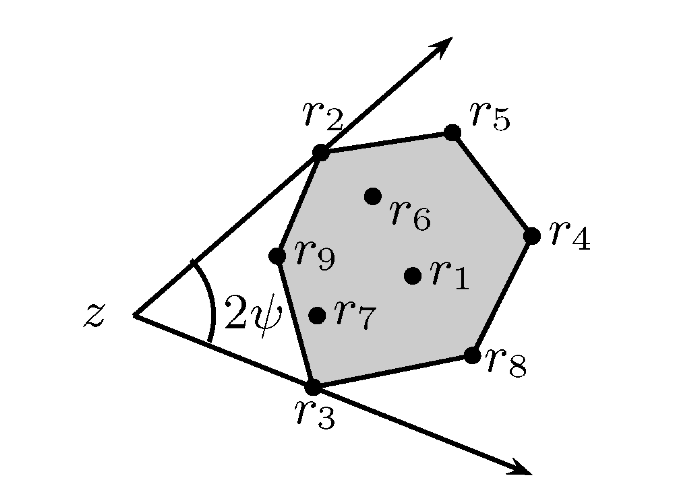
\includegraphics[width=0.5\textwidth]{fig_pb14.png}
	\caption{Figura 5. Unghiul de vizualizare \(2\psi\) al acoperirii convexe a mul\c{t}imii r\u{a}d\u{a}cinilor \(r_{1} , r_{2} , \cdots, r_{n}\)  lui \(P\left ( z \right )\), determin\u{a} parametrul \(\psi\) pe care \^{i}l g\u{a}sim \^{i}n rafinarea cantitativ\u{a} a lui Wilf a Teoremei Gauss-Lucas.}
\end{figure}

\end{problem}
\begin{proof}
Scriem \(r_{1} , r_{2} ,\cdots,r_{n}\) r\u{a}d\u{a}cinile lui \(P\) repetate \^{i}n func\c{t}ie de multiplicitatea lor \c{s}i pentru un \(z\) care se afl\u{a} \^{i}n afara acoperirii convexe \(H\) scriem \(z - r_{j}\) \^{i}n forma polar\u{a} \(z - r_{j} = \rho _{j}e^{i\theta j}\). Atunci avem
\begin{displaymath}
  \frac{1}{z - r_{j}} = \rho _{j}^{-1}e^{-\theta ji} , 1 \leq  j \leq  n,
\end{displaymath}
\c{s}i diferen\c{t}a \^{i}ntre argumentele \(\theta _{j}, 1 \leq j\leq n\) este mai mic\u{a} sau egal\u{a} cu \(2\psi\). Astfel, din Inegalitatea  MA-MG forma complex\u{a},avem
\begin{displaymath}
  \left ( \cos\psi  \right )\left | \frac{1}{z - r_{1}} \frac{1}{z - r_{2}}\cdots \frac{1}{z - r_{n}} \right|^{\frac{1}{n}} \leq  \frac{1}{n} \left | \sum_{j = 1}^{n}\frac{1}{z - r_{j}} \right |
\end{displaymath}
care \^{i}n termeni de \(P\) \c{s}i \({P}'\), se scrie c\u{a}
\begin{displaymath}
   \left | \frac{a_{n}}{P\left ( z \right )} \right |^{\frac{1}{n}}\leq \frac{1}{n\cos\psi }\left | \frac{{P}'\left ( z \right )}{P\left ( z \right )} \right |,  \text{pentru orice }z \notin H,
\end{displaymath}
 ceea ce doream s\u{a} demonstr\u{a}m.
\end{proof}

\begin{problem}
Dac\u{a} toate r\u{a}d\u{a}cinile polinomului \(P\left ( z \right ) = a_{n}z^{n} +\cdots +a_{1}z + a_{0}\) sunt con\c{t}inute \^{i}n discul unitate \(U= \left \{ z: \left | z \right |\leq 1 \right \}\), atunci
\begin{displaymath}
    n\left | a_{n} \right |^{\frac{1}{n}}\left | P\left ( z \right ) \right |^{\frac{\left ( n-1 \right )}{n}}\sqrt{1 - \left | z \right |^{-2}}\leq \left | {P}'\left ( z \right ) \right |, \text{pentru orice } z\notin U. \label{eq:2.17} \tag{2.17}
\end{displaymath}
\end{problem}
\begin{proof}
Dac\u{a} \(2\psi\) este unghiul de vizualizare determinat de \(U\) c\^{a}nd este privit din \(z \notin U\), atunci avem \(1 = \left | z \right |\sin\psi\), deci Teorema lui Pitagora ne spune c\u{a} \(\cos\psi = \left ( 1 - \left | z \right |^{-2} \right )^{\frac{1}{2}}\). Inegalitatea  \ref{eq:2.17} rezult\u{a} apoi direct din inegalitatea lui Wilf, \ref{eq:2.16}.
\end{proof}
\begin{problem}
Ar\u{a}ta\c{t}i c\u{a} dac\u{a} \(0 < r < 1\) \c{s}i dac\u{a} numerele complexe \(z_{1}, z_{2},...,z_{n}\) sunt \^{i}n discul \(D = \left \{ z: \left | z \right | \leq r\right \}\), atunci exist\u{a} \(z_{0} \in D\) astfel \^{i}nc\^{a}t
\begin{displaymath}
    \prod_{j = 1}^{n}\left ( 1 + z_{j} \right ) = \left ( 1 + z_{0} \right )^{n}.\label{eq:2.18} \tag{2.18}
\end{displaymath}
\end{problem}
\begin{proof}
Discul \(D_{0} = \left \{ z : \left | 1 - z \right |\leq 1 \right \}\) scris \^{i}n coordonate polare este
\begin{displaymath}
    \left \{ re^{i\theta }: 0 \leq r\leq 2\cos\theta , -\frac{\pi }{2}< \theta  < \frac{\pi }{2} \right \},
\end{displaymath}
deci pentru fiecare \(j\) putem scrie \(1 + z_{j}\) ca \(r_{j}e^{i\theta _{j}}\) unde \[-\frac{\pi }{2}< \theta  < \frac{\pi }{2},~r_{j}\leq 2\cos\theta _{j}.\]
 Rezult\u{a} imediat c\u{a} \[z_{0} = -1 + \left ( r_{1} r_{2}\cdots r_{n}\right )^{\frac{1}{n}}exp\left ( i\frac{\left ( \theta _{1} + \theta _{2} +....+ \theta _{n} \right )}{n} \right )\] este solu\c{t}ia ecua\c{t}iei lui Nievergelt \ref{eq:2.18} \c{s}i pentru a demonstra c\u{a} \(z_{0}\in D \) este suficient s\u{a} ar\u{a}t\u{a}m c\u{a} \(1 + z_{0}\in D_{0}\), echivalent, trebuie s\u{a} ar\u{a}t\u{a}m c\u{a}
\begin{displaymath}
    \left ( r_{1} r_{2} \cdots r_{n}\right )^{\frac{1}{n}}\leq 2\cos\left ( \frac{\theta _{1} + \theta _{2}+\cdots+\theta _{n}}{n} \right ) \label{eq:2.19} \tag{2.19}.
\end{displaymath}
Cum \(\left ( r_{1} r_{2} \cdots r_{n}\right )^{\frac{1}{n}}\) este marginit\u{a} de \(\left ( \left (2\cos\theta _{1}  \right )\left ( 2\cos\theta _{2} \right )\cdots \left (2\cos\theta _{n}  \right ) \right )^{\frac{1}{n}}\), este deci suficient s\u{a} ar\u{a}t\u{a}m c\u{a}
\begin{displaymath}
    \left ( \left (\cos\theta _{1}  \right )\left ( \cos\theta _{2} \right )\cdots \left (\cos\theta _{n}  \right ) \right )^{\frac{1}{n}}\leq \cos\left ( \frac{\theta _{1} + \theta _{2}+\cdots+\theta _{n}}{n} \right )
\end{displaymath}
\c{s}i aceasta rezult\u{a} din concavitatea lui \(f\left ( x \right ) = \log \left ( \cos x \right ) pe -\frac{\pi }{2}< \theta < \pi\) \^{i}mpreun\u{a} cu inegalitatea lui Jensen.
\end{proof}

\begin{problem} (Inegalitatea sumei ciclice a lui Shapiro)

Ar\u{a}ta\c{t}i c\u{a} pentru orice numere pozitive
 \(a_{1} , a_{2} , a_{3}\)  si \(  a_{4}\), avem inegalitatea
 \begin{displaymath}
     2\leq \frac{a_{1}}{a_{2} + a_{3}} + \frac{a_{2}}{a_{3} + a_{4}} + \frac{a_{3}}{a_{4} + a_{1}} + \frac{a_{4}}{a_{1} + a_{2}} \label{eq:2.20} \tag{2.20}
 \end{displaymath}
 \end{problem}
 \begin{remark}
De altfel,  Bushell (1994) ne ofer\u{a} o mul\c{t}ime de informa\c{t}ii despre inegalit\u{a}\c{t}i de forma
\begin{displaymath}
    \frac{n}{2} \leq \frac{x_{1}}{x_{2} + x_{3}} + \frac{x_{2}}{x_{3} + x_{4}} + \cdots+ \frac{x_{n - 1}}{x_{n} + x_{1}} + \frac{x_{n}}{x_{1} + x_{2}}.
\end{displaymath}
Se \c{s}tie c\u{a} aceast\u{a} inegalitate nu este adevarat\u{a} pentru  \(n\geq 25\), totu\c{s}i mul\c{t}imea precis\u{a} a valorilor lui n pentru care este adevarat\u{a}, nu a fost \^{i}nc\u{a} determinat\u{a}.
\end{remark}
\begin{proof}
O solu\c{t}ie frumoas\u{a} folosind inegalitatea lui Jensen pentru \(f\left ( x \right ) = \frac{1}{x}\) a fost dat\u{a} de Robert Israel \^{i}n grupul de \c{s}tiri sci.math \^{i}n 1999.

Dac\u{a} not\u{a}m \(S = a_{1} + a_{2} + a_{3} + a_{4}\) si \(C\) reprezint\u{a} suma din partea dreapt\u{a} a inegalit\u{a}\c{t}ii \ref{eq:2.18}, atunci Inegalitatea lui Jensen cu \(p_{j} = \frac{a_{j}}{S}\) \c{s}i
\[x_{1} = a_{2} + a_{3}, x_{2} = a_{3} + a_{4}, x_{3} = a_{4} + a_{1},~x_{4} = a_{1} + a_{2}\] conduce la
\[\frac{C}{S} \geq \left \{ \frac{D}{S} \right \}^{-1}\]
 sau \(C \geq \frac{S^{2}}{D}\), unde am notat
\begin{displaymath}
    D = a_{1}\left ( a_{2} + a_{3} \right ) + a_{2}\left ( a_{3} + a_{4} \right ) + a_{3}\left ( a_{4} + a_{1} \right ) + a_{4}\left ( a_{1} + a_{2} \right ).
\end{displaymath}
Acum, este simplu s\u{a} verific\u{a}m c\u{a}
\begin{displaymath}
    S^{2} - 2D = \left ( a_{1} - a_{3} \right )^{2} + \left ( a_{2} - a_{4} \right )^{2}> 0.
\end{displaymath}
Acest lucru este suficient pentru a completa solu\c{t}ia.
\end{proof}

\begin{problem} (Lema celor trei coarde)
Ar\u{a}ta\c{t}i c\u{a} dac\u{a} \(f : \left [ a,b \right ]  \to \mathbb{R}\) este convex\u{a} \c{s}i \(a <  x < b\), atunci avem
\begin{displaymath}
    \frac{f\left ( x \right ) - f\left ( a \right )}{x - a} \leq \frac{f\left ( b \right ) - f\left ( a \right )}{b - a} \leq  \frac{f\left ( b \right ) - f\left ( x \right )}{b - x}.   \label{eq:2.21}\tag{2.21}
\end{displaymath}
\end{problem}
\begin{proof}
Din convexitate avem
\begin{displaymath}
    x = \frac{b - x}{b - a}a + \frac{x - a}{b - a }b \Rightarrow f\left ( x \right ) \leq \frac{b - x}{b - a}f\left ( a \right ) + \frac{x - a}{b - a }f\left ( b \right )
\end{displaymath}
 deci, dup\u{a} sc\u{a}derea lui \(f\left ( a \right )\), va rezulta
 \begin{displaymath}
     f\left ( x \right ) - f\left ( a \right )\leq \frac{x - a}{b - a }\left \{ f\left ( b \right ) - f\left ( a \right ) \right \}. \label{eq:2.22} \tag{2.22}
 \end{displaymath}
Aceasta ne d\u{a} a doua inegalitate din \ref{eq:2.21} iar prima inegalitate se demonstreaz\u{a} \^{i}n acela\c{s}i mod.
\end{proof}

\chapter* {Concluzii}

Lucrarea de fa\c{t}\u{a} prezint\u{a} o scurt\u{a} prezentare a func\c{t}iior convexe, precum \c{s}i aplica\c{t}ii ale acestora.  Recunoa\c{s}terea func\c{t}iilor convexe ca o clas\u{a} de func\c{t}ii care trebuie studiat\u{a} poate fi urm\u{a}rit \^{i}n general p\^{a}n\u{a} la  J. L. W. V. Jensen \^{I}n orice caz, el nu a fost primul care a studiat funcţiile convexe. 

 Forma discret\u{a} a inegalit\u{a}\c{t}ii lui Jensen a fost demonstrat\u{a} pentru prima dat\u{a} de Hölder \^{i}n 1889, sub ipoteza c\u{a} derivata a doua este pozitiv\u{a}. Mai mult, Stolz a demonstrat \^{i}n 1893 c\u{a} fiecare punct de mijloc al func\c{t}ie continue \c{s}i convexe \(f : \left [ a,b \right ] \rightarrow \mathbb{R}\) are derivate la st\^{a}nga \c{s}i la dreapta \^{i}n fiecare punct al intervalului \(\left ( a,b \right )\). \^{I}n timp ce func\c{t}iile obi\c{s}nuite convexe sunt continue \^{i}n toate punctele interioare,  func\c{t}iile convexe ale punctului de mijloc pot fi discontinue peste tot. De fapt, privind \(\mathbb{R}\) ca un spa\c{t}iu vectorial \(\mathbb{Q}\) \c{s}i alegem o baz\u{a} \(\left ( b_{i} \right )_{i \in I}\) a lui \(\mathbb{R}\) peste \(\mathbb{Q}\), care este, o mul\c{t}ime maxim\u{a}, liniar independent\u{a}.
 
 Am putut vedea cum, Inegalitatea lui Young poate fi de asemnea ob\c{t}inut\u{a} ca o consecin\c{t}\u{a} a convexit\u{a}\c{t}ii stricte a func\c{t}iei exponen\c{t}iale. 
 
Cel de al doilea capitol, cuprinde aplica\c{t}ii ale func\c{t}iilor convexe \c{s}i anume Formula defectului lui Hölder. Aceasta este mai pu\c{t}in cunoscut\u{a} ca bine cunosscuta Inegalitatea a lui Hölder \c{s}i ofer\u{a} o m\u{a}sur\u{a} perfect natural\u{a} a diferen\c{t}ei dintre cele dou\u{a} p\u{a}r\c{t}i ale inegalit\u{a}\c{t}ii lui Jensen \c{s}i ne spune cum putem s\u{a} demonstr\u{a}m inegalitatea lui Jensen, ori de c\^{a}te ori putem verifica ipoteza suplimentar\u{a} 2.5, sau, \^{i}n cazul \^{i}n care aceasta se comport\u{a} ca o func\c{t}ie afin\u{a}, partea st\^{a}ng\u{a} a egalit\u{a}\c{t}ii 2.6 este egal\u{a} cu 0. 

De asemenea,printre probleme abordate se nun\u{a}r\u{a} cele \^{i}n care am aplicat  Inegalitatea lui Jensen, Inegalitatea ariei n-poligonului, Inegalit\u{a}\c{t}ile investi\c{t}ionale, Supraaditivitatea mediei geometrice - cu ajutorul Inegalit\u{a}\c{t}ii ui Jensen \c{s}i nu \^{i}n ultimul r\^{a}nd am abordat probleme care presupun criteriul derivatei a doua i teorema lui Rolle. 







\bibliographystyle{unsrt}
\setlength{\baselineskip}{\normalbaselineskip}
\setlength{\parskip}{0pt}
\bibliography{refs}
\end{document}














% \begin{problem} (Lema celor trei coarde)
% Ar\u{a}ta\c{t}i c\u{a} dac\u{a} \(f : \left [ a,b \right ]  \to \mathbb{R}\) este convex\u{a} \c{s}i \(a <  x < b\), atunci avem
% \begin{displaymath}
%     \frac{f\left ( x \right ) - f\left ( a \right )}{x - a} \leq \frac{f\left ( b \right ) - f\left ( a \right )}{b - a} \leq  \frac{f\left ( b \right ) - f\left ( x \right )}{b - x}.   \label{eq:2.21}\tag{2.21}
% \end{displaymath}
% \end{problem}
% \begin{remark}
% A\c{s}a cum ne sugereaz\u{a} urm\u{a}toarele dou\u{a} exerci\c{t}ii, aceast\u{a} limit\u{a} este cheia pentru c\^{a}teva dintre cele mai de baz\u{a} propriet\u{a}\c{t}i de regularitate ale func\c{t}iilor convexe.
% \end{remark}
% Prin interpolare \c{s}i convexitate avem
% \begin{displaymath}
%     x = \frac{b - x}{b - a}a + \frac{x - a}{b - a }b \Rightarrow f\left ( x \right ) \leq \frac{b - x}{b - a}f\left ( a \right ) + \frac{x - a}{b - a }f\left ( b \right )
% \end{displaymath}
%  deci, dup\u{a} scaderea lui \(f\left ( a \right )\), avem
%  \begin{displaymath}
%      f\left ( x \right ) - f\left ( a \right )\leq \frac{x - a}{b - a }\left \{ f\left ( b \right ) - f\left ( a \right ) \right \}. \label{eq:2.22} \tag{2.22}
%  \end{displaymath}
% Aceasta ne da a doua inegalitate a \ref{eq:2.21} iar cea de a doua este demonstrat\u{a} \^{i}n acela\c{s}i mod.


% Problema 21

% Aproape diferen\c{t}iabilitatea func\c{t}iilor convexe

% Folosind Lema celor trei coarde pentru a ar\u{a}ta c\u{a} pentru func\c{t}ia convex\u{a} \(f : \left [ a,b \right ]  \to \mathbb{R}\) si \(a< x< b\) exist\u{a} limite finite
% \begin{displaymath}
%     {f}'_{+} + \left ( x \right ) = \lim_{h  \to 0}\frac{f\left ( x + h \right ) - f\left ( x \right )}{h}
% \end{displaymath}
% \c{s}i
% \begin{displaymath}
%     {f}'_{-} + \left ( x \right ) = \lim_{h  \to 0}\frac{f\left ( x - h \right ) - f\left ( x \right )}{h}.
% \end{displaymath}
% Fie
% \begin{displaymath}
%     g\left ( h \right ) = \frac{\left \{ f\left ( x + h \right ) - f\left ( x \right ) \right \}}{h}
% \end{displaymath}
%  \c{s}i verific\u{a}m de la Lema celor trei coarde c\u{a} pentru \(0 < h_{1} < h_{2}\) avem \(g\left ( h_{1} \right )\leq g\left ( h_{2} \right )\). Mai departe lu\u{a}m \(y\) cu \(a <  y < x \) \c{s}i folosim Lema celor trei coarde pentru a verifica c\u{a}
%  \begin{displaymath}
%     -\infty < \frac{\left \{ f\left ( x \right ) - f\left ( y \right ) \right \}}{x - y}\geq g\left ( h \right )
%  \end{displaymath}
%  pentru orice \(h> 0\). Monotonitatea \c{s}i m\u{a}rginirea \(g\left ( h \right )\) garanteaz\u{a} faptul c\u{a} \(g\left ( h \right )\) are limit\u{a} finit\u{a} \^{i}n \(h \to 0\). Acest lucru ne ofer\u{a} prima jumatate a problemei, iar cea de a doua aproape identic.

% Problema 22

% Limitele de raport \c{s}i minoran\c{t}ii liniari

% Pentru func\c{t}iile convexe \(f : \left [ a,b \right ]  \to \mathbb{R}\) si \(a< x<y< b\), arata\c{t}i c\u{a} exist\u{a}
% \begin{displaymath}
%   {f}'_{-}\left ( x \right ) \leq  {f}'_{+}\left ( x \right ) \leq  \frac{f\left ( y \right ) - f\left ( x \right )}{y - x} \leq  {f}'_{-}\left ( y \right ) \leq  {f}'_{+}\left ( y \right ) \label{eq:2.23} \tag{2.23}
% \end{displaymath}

% \^{I}n particular, observ\u{a}m c\u{a} pentru orice
% \begin{displaymath}
%   \theta \in \left [ {f}'_{-}\left ( x \right ), {f}'_{+}\left ( x \right ) \right ],
% \end{displaymath}
%  avem limita
%  \begin{displaymath}
% (f\left ( y \right ) \geq  f\left ( x \right ) + \left ( y - x \right )\theta \text{pentru orice  }y\in \left [ a,b \right ]. \label{eq:2.24} \tag{2.24}
%  \end{displaymath}

% Limita inferioar\u{a} liniar\u{a} \ref{eq:2.22} este mai eficient\u{a} dec\^{a}t sugereaz\u{a} simplitatea sa \c{s}i are c\^{a}teva consecin\c{t}e notabile.
% Aceasta este doar o lucrare mai la \^{i}ndem\^{a}n\u{a} a Teoremei celor trei coarde care ne d\u{a} pentru \(0< s\) \c{s}i \(0< t\) cu \(y - s \in I\) si \(y + t  \in I\) faptul c\u{a}
% \begin{displaymath}
%   \frac{f\left ( y \right ) - f\left ( y - s \right )}{s}\leq \frac{f\left ( y + t \right ) - f\left ( y \right )}{t}.
% \end{displaymath}
%  De la exerci\c{t}iul 21 avem acele limite finite ca \(s,t \to 0\), \c{s}i aceste limite sunt \({f}'_{-}\left ( y \right )\) \c{s}i respectiv \({f}'_{+}\left ( y \right )\). Acest lucru ne ofer\u{a} faptul c\u{a} \({f}'_{-}\left ( y \right )\leq {f}'_{+}\left ( y \right )\) \c{s}i celelalte limite nu sunt mai grele. Identic, limita \({f}'_{-}\left ( y \right )\leq {f}'_{+}\left ( y \right )\) poate fi privit\u{a} ca o versiune infim\u{a} a Lemei celor trei coarde.
% Pentru \(a < x \leq s\leq t\leq y<  b\) \c{s}i \( M = max\left \{ \left | {f}'_{+} \left ( x \right )\right |,\left | {f}'_{-} \left ( y \right )\right |  \right \}\) limita \ref{eq:2.21} ne ofer\u{a} \(\left | f\left ( t \right ) - f\left ( s \right ) \right |\leq M\left | t - s \right |\), care este mai mult dec\^{a}t aveam nevoie pentru a spune ca f este conutinu\u{a}.


